% Options for packages loaded elsewhere
% Options for packages loaded elsewhere
\PassOptionsToPackage{unicode}{hyperref}
\PassOptionsToPackage{hyphens}{url}
\PassOptionsToPackage{dvipsnames,svgnames,x11names}{xcolor}
%
\documentclass[
  9pt,
  letterpaper,
  DIV=11,
  numbers=noendperiod]{scrartcl}
\usepackage{xcolor}
\usepackage{amsmath,amssymb}
\setcounter{secnumdepth}{-\maxdimen} % remove section numbering
\usepackage{iftex}
\ifPDFTeX
  \usepackage[T1]{fontenc}
  \usepackage[utf8]{inputenc}
  \usepackage{textcomp} % provide euro and other symbols
\else % if luatex or xetex
  \usepackage{unicode-math} % this also loads fontspec
  \defaultfontfeatures{Scale=MatchLowercase}
  \defaultfontfeatures[\rmfamily]{Ligatures=TeX,Scale=1}
\fi
\usepackage{lmodern}
\ifPDFTeX\else
  % xetex/luatex font selection
\fi
% Use upquote if available, for straight quotes in verbatim environments
\IfFileExists{upquote.sty}{\usepackage{upquote}}{}
\IfFileExists{microtype.sty}{% use microtype if available
  \usepackage[]{microtype}
  \UseMicrotypeSet[protrusion]{basicmath} % disable protrusion for tt fonts
}{}
\makeatletter
\@ifundefined{KOMAClassName}{% if non-KOMA class
  \IfFileExists{parskip.sty}{%
    \usepackage{parskip}
  }{% else
    \setlength{\parindent}{0pt}
    \setlength{\parskip}{6pt plus 2pt minus 1pt}}
}{% if KOMA class
  \KOMAoptions{parskip=half}}
\makeatother
% Make \paragraph and \subparagraph free-standing
\makeatletter
\ifx\paragraph\undefined\else
  \let\oldparagraph\paragraph
  \renewcommand{\paragraph}{
    \@ifstar
      \xxxParagraphStar
      \xxxParagraphNoStar
  }
  \newcommand{\xxxParagraphStar}[1]{\oldparagraph*{#1}\mbox{}}
  \newcommand{\xxxParagraphNoStar}[1]{\oldparagraph{#1}\mbox{}}
\fi
\ifx\subparagraph\undefined\else
  \let\oldsubparagraph\subparagraph
  \renewcommand{\subparagraph}{
    \@ifstar
      \xxxSubParagraphStar
      \xxxSubParagraphNoStar
  }
  \newcommand{\xxxSubParagraphStar}[1]{\oldsubparagraph*{#1}\mbox{}}
  \newcommand{\xxxSubParagraphNoStar}[1]{\oldsubparagraph{#1}\mbox{}}
\fi
\makeatother

\usepackage{color}
\usepackage{fancyvrb}
\newcommand{\VerbBar}{|}
\newcommand{\VERB}{\Verb[commandchars=\\\{\}]}
\DefineVerbatimEnvironment{Highlighting}{Verbatim}{commandchars=\\\{\}}
% Add ',fontsize=\small' for more characters per line
\usepackage{framed}
\definecolor{shadecolor}{RGB}{241,243,245}
\newenvironment{Shaded}{\begin{snugshade}}{\end{snugshade}}
\newcommand{\AlertTok}[1]{\textcolor[rgb]{0.68,0.00,0.00}{#1}}
\newcommand{\AnnotationTok}[1]{\textcolor[rgb]{0.37,0.37,0.37}{#1}}
\newcommand{\AttributeTok}[1]{\textcolor[rgb]{0.40,0.45,0.13}{#1}}
\newcommand{\BaseNTok}[1]{\textcolor[rgb]{0.68,0.00,0.00}{#1}}
\newcommand{\BuiltInTok}[1]{\textcolor[rgb]{0.00,0.23,0.31}{#1}}
\newcommand{\CharTok}[1]{\textcolor[rgb]{0.13,0.47,0.30}{#1}}
\newcommand{\CommentTok}[1]{\textcolor[rgb]{0.37,0.37,0.37}{#1}}
\newcommand{\CommentVarTok}[1]{\textcolor[rgb]{0.37,0.37,0.37}{\textit{#1}}}
\newcommand{\ConstantTok}[1]{\textcolor[rgb]{0.56,0.35,0.01}{#1}}
\newcommand{\ControlFlowTok}[1]{\textcolor[rgb]{0.00,0.23,0.31}{\textbf{#1}}}
\newcommand{\DataTypeTok}[1]{\textcolor[rgb]{0.68,0.00,0.00}{#1}}
\newcommand{\DecValTok}[1]{\textcolor[rgb]{0.68,0.00,0.00}{#1}}
\newcommand{\DocumentationTok}[1]{\textcolor[rgb]{0.37,0.37,0.37}{\textit{#1}}}
\newcommand{\ErrorTok}[1]{\textcolor[rgb]{0.68,0.00,0.00}{#1}}
\newcommand{\ExtensionTok}[1]{\textcolor[rgb]{0.00,0.23,0.31}{#1}}
\newcommand{\FloatTok}[1]{\textcolor[rgb]{0.68,0.00,0.00}{#1}}
\newcommand{\FunctionTok}[1]{\textcolor[rgb]{0.28,0.35,0.67}{#1}}
\newcommand{\ImportTok}[1]{\textcolor[rgb]{0.00,0.46,0.62}{#1}}
\newcommand{\InformationTok}[1]{\textcolor[rgb]{0.37,0.37,0.37}{#1}}
\newcommand{\KeywordTok}[1]{\textcolor[rgb]{0.00,0.23,0.31}{\textbf{#1}}}
\newcommand{\NormalTok}[1]{\textcolor[rgb]{0.00,0.23,0.31}{#1}}
\newcommand{\OperatorTok}[1]{\textcolor[rgb]{0.37,0.37,0.37}{#1}}
\newcommand{\OtherTok}[1]{\textcolor[rgb]{0.00,0.23,0.31}{#1}}
\newcommand{\PreprocessorTok}[1]{\textcolor[rgb]{0.68,0.00,0.00}{#1}}
\newcommand{\RegionMarkerTok}[1]{\textcolor[rgb]{0.00,0.23,0.31}{#1}}
\newcommand{\SpecialCharTok}[1]{\textcolor[rgb]{0.37,0.37,0.37}{#1}}
\newcommand{\SpecialStringTok}[1]{\textcolor[rgb]{0.13,0.47,0.30}{#1}}
\newcommand{\StringTok}[1]{\textcolor[rgb]{0.13,0.47,0.30}{#1}}
\newcommand{\VariableTok}[1]{\textcolor[rgb]{0.07,0.07,0.07}{#1}}
\newcommand{\VerbatimStringTok}[1]{\textcolor[rgb]{0.13,0.47,0.30}{#1}}
\newcommand{\WarningTok}[1]{\textcolor[rgb]{0.37,0.37,0.37}{\textit{#1}}}

\usepackage{longtable,booktabs,array}
\usepackage{calc} % for calculating minipage widths
% Correct order of tables after \paragraph or \subparagraph
\usepackage{etoolbox}
\makeatletter
\patchcmd\longtable{\par}{\if@noskipsec\mbox{}\fi\par}{}{}
\makeatother
% Allow footnotes in longtable head/foot
\IfFileExists{footnotehyper.sty}{\usepackage{footnotehyper}}{\usepackage{footnote}}
\makesavenoteenv{longtable}
\usepackage{graphicx}
\makeatletter
\newsavebox\pandoc@box
\newcommand*\pandocbounded[1]{% scales image to fit in text height/width
  \sbox\pandoc@box{#1}%
  \Gscale@div\@tempa{\textheight}{\dimexpr\ht\pandoc@box+\dp\pandoc@box\relax}%
  \Gscale@div\@tempb{\linewidth}{\wd\pandoc@box}%
  \ifdim\@tempb\p@<\@tempa\p@\let\@tempa\@tempb\fi% select the smaller of both
  \ifdim\@tempa\p@<\p@\scalebox{\@tempa}{\usebox\pandoc@box}%
  \else\usebox{\pandoc@box}%
  \fi%
}
% Set default figure placement to htbp
\def\fps@figure{htbp}
\makeatother


% definitions for citeproc citations
\NewDocumentCommand\citeproctext{}{}
\NewDocumentCommand\citeproc{mm}{%
  \begingroup\def\citeproctext{#2}\cite{#1}\endgroup}
\makeatletter
 % allow citations to break across lines
 \let\@cite@ofmt\@firstofone
 % avoid brackets around text for \cite:
 \def\@biblabel#1{}
 \def\@cite#1#2{{#1\if@tempswa , #2\fi}}
\makeatother
\newlength{\cslhangindent}
\setlength{\cslhangindent}{1.5em}
\newlength{\csllabelwidth}
\setlength{\csllabelwidth}{3em}
\newenvironment{CSLReferences}[2] % #1 hanging-indent, #2 entry-spacing
 {\begin{list}{}{%
  \setlength{\itemindent}{0pt}
  \setlength{\leftmargin}{0pt}
  \setlength{\parsep}{0pt}
  % turn on hanging indent if param 1 is 1
  \ifodd #1
   \setlength{\leftmargin}{\cslhangindent}
   \setlength{\itemindent}{-1\cslhangindent}
  \fi
  % set entry spacing
  \setlength{\itemsep}{#2\baselineskip}}}
 {\end{list}}
\usepackage{calc}
\newcommand{\CSLBlock}[1]{\hfill\break\parbox[t]{\linewidth}{\strut\ignorespaces#1\strut}}
\newcommand{\CSLLeftMargin}[1]{\parbox[t]{\csllabelwidth}{\strut#1\strut}}
\newcommand{\CSLRightInline}[1]{\parbox[t]{\linewidth - \csllabelwidth}{\strut#1\strut}}
\newcommand{\CSLIndent}[1]{\hspace{\cslhangindent}#1}



\setlength{\emergencystretch}{3em} % prevent overfull lines

\providecommand{\tightlist}{%
  \setlength{\itemsep}{0pt}\setlength{\parskip}{0pt}}



 


\usepackage{booktabs}
\usepackage{longtable}
\usepackage{array}
\usepackage{multirow}
\usepackage{wrapfig}
\usepackage{float}
\usepackage{colortbl}
\usepackage{pdflscape}
\usepackage{tabu}
\usepackage{threeparttable}
\usepackage{threeparttablex}
\usepackage[normalem]{ulem}
\usepackage{makecell}
\usepackage{xcolor}
\renewcommand{\baselinestretch}{1.1}
\usepackage{graphicx}
\usepackage{xcolor}
\usepackage{amsmath,amssymb}
\usepackage{booktabs}
\usepackage{longtable}
\usepackage{array}
\usepackage{multirow}
\usepackage{makecell}
\usepackage{pdflscape}
\usepackage{float}
\usepackage{fancyhdr}
\KOMAoption{captions}{tableheading}
\makeatletter
\@ifpackageloaded{caption}{}{\usepackage{caption}}
\AtBeginDocument{%
\ifdefined\contentsname
  \renewcommand*\contentsname{Table of contents}
\else
  \newcommand\contentsname{Table of contents}
\fi
\ifdefined\listfigurename
  \renewcommand*\listfigurename{List of Figures}
\else
  \newcommand\listfigurename{List of Figures}
\fi
\ifdefined\listtablename
  \renewcommand*\listtablename{List of Tables}
\else
  \newcommand\listtablename{List of Tables}
\fi
\ifdefined\figurename
  \renewcommand*\figurename{Figure}
\else
  \newcommand\figurename{Figure}
\fi
\ifdefined\tablename
  \renewcommand*\tablename{Table}
\else
  \newcommand\tablename{Table}
\fi
}
\@ifpackageloaded{float}{}{\usepackage{float}}
\floatstyle{ruled}
\@ifundefined{c@chapter}{\newfloat{codelisting}{h}{lop}}{\newfloat{codelisting}{h}{lop}[chapter]}
\floatname{codelisting}{Listing}
\newcommand*\listoflistings{\listof{codelisting}{List of Listings}}
\makeatother
\makeatletter
\makeatother
\makeatletter
\@ifpackageloaded{caption}{}{\usepackage{caption}}
\@ifpackageloaded{subcaption}{}{\usepackage{subcaption}}
\makeatother
\usepackage{bookmark}
\IfFileExists{xurl.sty}{\usepackage{xurl}}{} % add URL line breaks if available
\urlstyle{same}
\hypersetup{
  pdftitle={Longitudinal Analysis of Alzheimer's Disease Progression: Modeling Cognitive and Psychiatric Trajectories with Informative Dropout},
  pdfauthor={Anita Kerubo Ogero (2469491); Okolie Tess Eucharia (2468507); Moses Mburu (2469245); Dorothy Chepkoech (2469284)},
  colorlinks=true,
  linkcolor={blue},
  filecolor={Maroon},
  citecolor={Blue},
  urlcolor={Blue},
  pdfcreator={LaTeX via pandoc}}


\title{Longitudinal Analysis of Alzheimer's Disease Progression:
Modeling Cognitive and Psychiatric Trajectories with Informative
Dropout}
\author{Anita Kerubo Ogero (2469491) \and Okolie Tess Eucharia
(2468507) \and Moses Mburu (2469245) \and Dorothy Chepkoech (2469284)}
\date{}
\begin{document}
\maketitle


\subsection{Abstract}\label{abstract}

Alzheimer's disease is characterised by progressive cognitive and
neuropsychiatric decline, but longitudinal analysis is complicated by
dropout and non-random missingness. We analysed up to six annual
follow-up measurements of BPRS (psychiatric symptoms) and CDR-SB
(cognitive--functional status) in an Alzheimer cohort, focusing on
missingness, disease trajectories, and baseline predictors. Missingness
was monotone and strongly related to baseline severity, supporting a
missing-at-random (MAR) assumption rather than missing completely at
random. For BPRS, a linear mixed model showed a clear increase over time
\((\approx7.2 points/year, p < 0.001)\), with higher symptom levels
among patients who were older, had poorer ADL, lived in nursing homes,
or were not employed. Baseline CDR-SB moderated BPRS progression, with
more impaired patients showing slower subsequent worsening. For severe
CDR-SB (CDR-SB \textgreater{} 10), logistic mixed models and weighted
GEE revealed increasing risk over time and an important role for tau
PET. A \(\delta\)-shift pattern-mixture sensitivity analysis indicated
that these conclusions were robust to plausible MNAR departures.
Clinically, this suggests our findings give a reliable picture of how
psychiatric and cognitive problems progress in Alzheimer's disease,
despite substantial loss to follow-up.

\subsection{Introduction}\label{introduction}

Alzheimer's disease is the most common cause of dementia and is a
progressive neurodegenerative condition that leads to worsening
cognition, neuropsychiatric symptoms, and day-to-day functioning
(\citeproc{ref-scheltens2016ad}{Scheltens \emph{et al.}, 2016}).
Dementia is a major global health burden, World Health Organization
(WHO) estimates that 57 million people were living with dementia in
2021, with nearly 10 million new cases each year, and the burden falls
mainly on older adults (\citeproc{ref-who_dementia}{World Health
Organization, 2025}). Because symptoms change gradually and
heterogeneously across patients, longitudinal studies are central for
describing average progression, quantifying between patient differences,
and identifying baseline factors linked to faster or slower
deterioration. In Alzheimer research and clinical trials, cognitive
functional progression is commonly tracked with the Clinical Dementia
Rating--Sum of Boxes (CDR-SB), which captures both cognitive and
functional impairment and tends to worsen in a roughly steady way over
follow-up in symptomatic disease
(\citeproc{ref-cedarbaum2013cdrsb}{Cedarbaum \emph{et al.}, 2013};
\citeproc{ref-williams2013cdrsb}{Williams \emph{et al.}, 2013}).
Psychiatric symptom burden can be summarised using clinician-rated
scales such as the Brief Psychiatric Rating Scale (BPRS), which has been
applied in Alzheimer populations to characterise behavioural and
psychological symptoms (\citeproc{ref-ownby1994bprs}{Ownby \emph{et
al.}, 1994}).

In this study, we analyse longitudinal data from a cohort of newly
diagnosed patients recruited across several clinical centres and
followed annually for up to six years. The main outcomes of interest
include repeatedly measured psychiatric symptoms, assessed using the
Brief Psychiatric Rating Scale (BPRS), and cognitive--functional status,
summarised using the Clinical Dementia Rating Sum of Boxes (CDR-SB).
Biomarkers related to Alzheimer's pathology, including amyloid and tau
positron emission tomography (PET) measures, were obtained alongside
baseline demographic and clinical characteristics, providing a rich
multivariate dataset for studying disease progression.

A key challenge in such long-term follow-up studies is the presence of
missing data due to dropout, which is particularly common in elderly and
clinically vulnerable populations. When missingness is associated with
disease severity or functional decline, the observed data may become
increasingly selective over time, leading to biased estimates if naive
complete-case approaches are used. As emphasised in the longitudinal
missing-data literature, valid inference requires statistical models
that can account for informative dropout or missingness mechanisms that
depend on observed patient history rather than future unobserved
outcomes (\citeproc{ref-molenberghs2004incomplete}{Molenberghs \emph{et
al.}, 2004}). This study therefore investigates appropriate longitudinal
modelling approaches that remain valid under realistic missingness
assumptions and explores the robustness of key clinical conclusions to
deviations from the missing at random framework.

The objectives of this analysis are four. First, to describe and explore
the extent and patterns of missing data over follow-up. As part of this,
we assess whether the data are consistent with missing completely at
random (MCAR) by examining associations between missingness and observed
patient characteristics and earlier outcomes. Second, to describe and
model the evolution of psychiatric symptom severity (BPRS) over time and
how it relates to baseline patient characteristics and disease severity,
using methods that account for correlation between repeated measurements
within the same patient and unbalanced follow-up
(\citeproc{ref-laird1982random}{Laird and Ware, 1982}). Third, to model
how the probability of being in the worst cognitive category (CDR-SB
\textgreater{} 10) changes over time and how it relates to baseline
characteristics and biomarkers, using marginal and subject-specific
frameworks for longitudinal binary outcomes
(\citeproc{ref-liang1986longitudinal}{Liang and Zeger, 1986}). Fourth,
since the missing-at-random (MAR) assumption cannot be verified from the
observed data and MAR and missing not at random (MNAR) mechanisms can
lead to the same observed patterns, we perform a sensitivity analysis
that explores clinically plausible departures from MAR toward missing
not at random (MNAR) for the continuous BPRS outcome
(\citeproc{ref-little1993pattern}{Little, 1993}).

\subsection{Methodology}\label{methodology}

\subsubsection{Study design, outcomes, and
covariates}\label{study-design-outcomes-and-covariates}

We analysed data from a multicentre cohort of patients diagnosed with
Alzheimer's disease who were assessed annually for up to six years.
Psychiatric symptom severity was measured repeatedly using the Brief
Psychiatric Rating Scale (BPRS). Cognitive status was measured using the
Clinical Dementia Rating Sum of Boxes (CDR-SB). Two positron emission
tomography biomarkers were also assessed annually, amyloid positron
emission tomography (amyloid PET) and tau positron emission tomography
(tau PET).

For the cognitive endpoint, the continuous CDR-SB score was dichotomised
to define a clinically severe category:

\[
Z_{ij} = \mathbb{I}\!\left(\mathrm{CDR\text{-}SB}_{ij} > 10\right),
\]

where \(i=1,\dots,N\) indexes patients and \(j=0,\dots,J\) indexes the
scheduled annual visits, with \(j=0\) baseline.

Baseline characteristics included age, sex, education, body mass index,
functional status (activities of daily living), employment status, and
living situation. These are denoted collectively by \(X_i\). Baseline
disease severity measures are denoted by \(S_i\) (including baseline
CDR-SB, and baseline biomarker measures where relevant).

\subsubsection{Analysis objectives}\label{analysis-objectives}

The analysis had four linked objectives:

\begin{enumerate}
\def\labelenumi{\arabic{enumi}.}
\tightlist
\item
  Describe the amount and structure of missing follow-up data and assess
  whether missingness depends on observed outcomes or covariates.
\item
  Characterise the average evolution of BPRS over time and how it
  relates to baseline characteristics and baseline disease severity.
\item
  Characterise the evolution over time of the dichotomised cognitive
  outcome based on CDR-SB.
\item
  Assess how sensitive the BPRS conclusions are to departures from the
  primary missing-data assumption.
\end{enumerate}

\subsubsection{Missing follow-up data}\label{missing-follow-up-data}

\paragraph{Notation for missingness}\label{notation-for-missingness}

Let \(Y_{ij}\) denote BPRS at visit \(j\) for patient \(i\).

\[
R_{ij} =
\begin{cases}
1, & \text{if } Y_{ij} \text{ is observed}, \\
0, & \text{if } Y_{ij} \text{ is missing}.
\end{cases}
\]

Let \(R_i=(R_{i0},\dots,R_{iJ})\) denote a patient's observation
pattern, and split the full outcome vector as
\(Y_i=(Y_i^{obs},Y_i^{mis})\).

\paragraph{Describing missingness
patterns}\label{describing-missingness-patterns}

Missingness patterns were first characterised descriptively to determine
whether dropout followed a monotone structure or whether intermittent
missingness occurred. For each subject, the last observed visit was
defined as

\[
t_i = \max\{j : R_{ij}=1\}.
\]

A subject was classified as exhibiting monotone dropout if \(R_{ij}=1\)
for all \(j \le t_i\) and \(R_{ij}=0\) for all \(j > t_i\). Non-monotone
(intermittent) missingness was defined as the presence of at least one
missing observation followed by a later observed measurement, i.e.~the
pattern is non-monotone if there exist \(j<k\) such that \(R_{ij}=0\)
and \(R_{ik}=1\).

These classifications were summarised using (i) the distribution of
\(t_i\) (retention over time), (ii) the proportion missing at each visit
\(j\), and (iii) the frequency of intermittent gaps within \(R_i\).

\paragraph{Assessing dependence of missingness on observed data (showing
data are not
MCAR)}\label{assessing-dependence-of-missingness-on-observed-data-showing-data-are-not-mcar}

We examined whether missingness is plausibly independent of observed
information (more consistent with MCAR) or related to observed disease
severity and covariates (supporting a MAR working assumption). This
included descriptive comparisons (for example, baseline BPRS by the
number of missed follow-up visits) and a discrete-time model for
dropout. The aim is to demonstrate that missingness is not consistent
with a completely random observation process and to motivate methods
that remain appropriate when dropout depends on observed history
(\citeproc{ref-molenberghs2004incomplete}{Molenberghs \emph{et al.},
2004}).

A convenient way to formalise dropout is to model the probability of
becoming missing at the next visit among those observed at the current
visit. Defined as:

\[
D_{i,j+1} = 1 - R_{i,j+1},
\]

and fit a logistic model of the form

\[
\Pr(D_{i,j+1}=1 \mid \mathcal{H}_{ij})
=
\operatorname{logit}^{-1}\!\left(
\alpha_0 + \alpha_1 Y_{ij} + \alpha_2^\top X_i + \alpha_3 j
\right),
\]

where \(\mathcal{H}_{ij}\) denotes the observed history up to visit
\(j\).

If dropout is associated with observed outcomes or covariates, this
argues against MCAR. Diggle and Kenward called this ``random dropout''
(dropout depending on observed history), for which likelihood-based
inference for the measurement model can proceed without explicitly
modelling the dropout process, provided standard
ignorability/distinct-parameter conditions hold
(\citeproc{ref-diggle1994informative}{Diggle and Kenward, 1994}).

\paragraph{Handling missing data in longitudinal
models}\label{handling-missing-data-in-longitudinal-models}

\subparagraph{Complete case analysis}\label{complete-case-analysis}

Complete case analysis restricts the analysis to patients with a fully
observed BPRS profile across all scheduled visits. In long follow-up
studies, this can remove a large proportion of the cohort and shifts the
analysis toward patients who remain under observation. When dropout is
related to disease course (for example, patients with worse psychiatric
symptoms or faster deterioration being more likely to miss later
visits), the complete-case estimate of the BPRS trajectory reflects the
evolution among stayers rather than the evolution in the full cohort. In
that setting, the average yearly change in BPRS can be biased because it
is estimated from a selected subgroup, and precision is reduced because
many observed BPRS measurements are discarded
(\citeproc{ref-molenberghs2004incomplete}{Molenberghs \emph{et al.},
2004}).

\subparagraph{Last observation carried forward (LOCF) and related
single-imputation
rules}\label{last-observation-carried-forward-locf-and-related-single-imputation-rules}

LOCF replaces each missing BPRS/CDR-SB value after dropout with the last
observed BPRS/CDR-SB score for that patient. For a progressive
condition, this effectively assumes that a patient's psychiatric symptom
level stays constant after the last attended visit. In terms of BPRS
evolution, LOCF tends to flatten the estimated mean trajectory at later
follow-up because patients who drop out contribute repeated copies of
their last score rather than a plausible continued change. This can lead
to underestimation (or distortion) of the average change over time, and
it treats imputed values as if they were observed when estimating
uncertainty, which can make confidence intervals look too narrow
(\citeproc{ref-molenberghs2004incomplete}{Molenberghs \emph{et al.},
2004}).

\subparagraph{Multiple imputation (MI)}\label{multiple-imputation-mi}

Multiple imputation treats the missing outcomes as additional unknown
quantities and replaces each missing value with \(m\) plausible draws
from an imputation model. Each imputed dataset is analysed using the
same substantive model, and results are then combined using Rubin's
rules so that standard errors reflect both within-imputation variability
and the extra uncertainty due to missingness.

Let \(\hat\theta^{(k)}\) and
\(\widehat{\mathrm{Var}}(\hat\theta^{(k)})\) denote the estimate and its
variance from imputed dataset \(k=1,\dots,m\). The pooled estimate is

\[
\bar\theta = \frac{1}{m}\sum_{k=1}^m \hat\theta^{(k)}.
\]

Define the within-imputation variance

\[
\bar U = \frac{1}{m}\sum_{k=1}^m \widehat{\mathrm{Var}}(\hat\theta^{(k)}),
\]

and the between-imputation variance

\[
B = \frac{1}{m-1}\sum_{k=1}^m \left(\hat\theta^{(k)}-\bar\theta\right)^2.
\]

The total variance is

\[
T = \bar U + \left(1+\frac{1}{m}\right)B.
\]

Multiple Imputation can be used for longitudinal outcomes by specifying
an imputation model that reflects the repeated-measures structure (time
trends, within-patient correlation, and key interactions). In practice,
when the proportion missing becomes large (in this study, missingness
reaches approximately 60\% at later follow-up), MI can become more
sensitive to imputation-model specification because a larger fraction of
the information about late follow-up trajectories is coming from
modelling assumptions rather than directly observed data. Simulation
work has shown that the amount of information that can be recovered by
MI decreases as missingness increases, and that careful model
specification becomes increasingly important at high levels of
missingness (\citeproc{ref-leecarlin2012mi}{Lee and Carlin, 2012}).

For these reasons, multiple imputation (MI) was not used as the primary
analysis strategy here. Instead, we relied on likelihood-based mixed
models for the main longitudinal analyses under a working MAR
assumption, and we used a sensitivity analysis to quantify how
conclusions change under departures from MAR.

\subparagraph{Likelihood-based approaches (primary analyses under a
working MAR
assumption)}\label{likelihood-based-approaches-primary-analyses-under-a-working-mar-assumption}

Our primary longitudinal models for BPRS (LMM) and for the dichotomised
CDR-SB endpoint (GLMM) are likelihood-based. Under MAR, missingness
depends only on observed information and not on unobserved outcomes:

\[
p(R_i \mid Y_i, X_i)=p(R_i \mid Y_i^{\mathrm{obs}}, X_i).
\]

Under standard ignorability conditions most importantly, that parameters
of the measurement model and the missingness model are distinct
likelihood inference based on the observed-data likelihood yields valid
estimation for the outcome-model parameters without requiring a fully
specified joint model for dropout
(\citeproc{ref-rubin1976inference}{Rubin, 1976};
\citeproc{ref-molenberghs2004incomplete}{Molenberghs \emph{et al.},
2004}). MAR cannot be confirmed from the observed data, so we
complemented the primary continuous-outcome analysis with a sensitivity
analysis that checks clinically plausible departures from MAR.

\subsubsection{Longitudinal models}\label{longitudinal-models}

\paragraph{Continuous outcome (BPRS): linear mixed effects model
(LMM)}\label{continuous-outcome-bprs-linear-mixed-effects-model-lmm}

This model describes how psychiatric symptom severity (BPRS) changes
over time in the cohort, while allowing different patients to start at
different symptom levels and to change at different rates. It accounts
for within-patient correlation from repeated measurements and
accommodates unequal follow-up due to dropout.

To model the BPRS trajectory, we used the linear mixed effects model
specification from Homework 1: \[
\begin{aligned}
\mathrm{BPRS}_{it} &= (\beta_0 + b_{0i} + u_{0j}) + (\beta_1 + b_{1i})\,\mathrm{time}_{it} \\
&\quad + \beta_2\,\mathrm{sex}_i + \beta_3\,\mathrm{age}_i + \beta_4\,\mathrm{bmi}_i + \beta_5\,\mathrm{job}_i \\
&\quad + \beta_6\,\mathrm{adl}_i + \beta_7\,\mathrm{wzc}_i + \beta_8\,\mathrm{CDR\text{-}SB}_{i0} \\
&\quad + \beta_9\!\left(\mathrm{time}_{it}\cdot \mathrm{CDR\text{-}SB}_{i0}\right) + \varepsilon_{it}.
\end{aligned}
\]

\textbf{fixed effects}

\begin{itemize}
\tightlist
\item
  \(\beta_0\) is the cohort-average baseline BPRS for a reference
  patient (given the covariate coding), before adding patient- and
  centre-level deviations.
\item
  \(\beta_1\) is the cohort-average yearly change in BPRS. A positive
  value indicates worsening psychiatric symptoms on average over time,
  while a negative value indicates improvement.
\item
  \(\beta_2,\dots,\beta_7\) represent average differences in BPRS
  associated with baseline characteristics (sex, age, BMI, employment
  status, activities of daily living, and living situation), holding the
  other covariates fixed.
\item
  \(\beta_8\) quantifies the association between baseline
  cognitive/functional severity (baseline CDR-SB) and baseline
  psychiatric symptom severity (BPRS).
\item
  \(\beta_9\) captures effect modification of the time trend by baseline
  CDR-SB. For example, if \(\beta_9>0\), patients with higher baseline
  CDR-SB tend to show a faster increase in BPRS over follow-up.
\end{itemize}

The model includes patient-specific random effects collected in
\(b_i=(b_{0i},b_{1i})^\top\), where \(b_{0i}\) represents the patient's
deviation from the cohort-average baseline BPRS and \(b_{1i}\)
represents the patient's deviation from the cohort-average yearly
change. The term \(u_{0j}\) is a centre/trial-specific random intercept
for centre/trial \(j\), capturing systematic baseline differences
between centres.

The random effects and residual errors are assumed to follow:

\[
\begin{pmatrix}
b_{0i} \\
b_{1i}
\end{pmatrix}
\sim
N\!\left(
\begin{pmatrix}
0 \\
0
\end{pmatrix},
D
\right),
\qquad
u_{0j} \sim N(0,\sigma^2_{\text{trial}}),
\qquad
\varepsilon_{it} \sim N(0,\sigma^2).
\]

Here, \(D\) quantifies between-patient variability in baseline BPRS and
in progression rate and allows correlation between them. The residual
term \(\varepsilon_{it}\) captures within-patient fluctuations and
measurement error around the patient-specific trajectory.

This likelihood-based model uses all available BPRS measurements and
supports inference under the working MAR/ignorability conditions
described earlier (\citeproc{ref-molenberghs2004incomplete}{Molenberghs
\emph{et al.}, 2004}).

\paragraph{Binary outcome (CDR-SB \textgreater{} 10): logistic
Generalized Linear Mixed Model (GLMM)
(subject-specific)}\label{binary-outcome-cdr-sb-10-logistic-generalized-linear-mixed-model-glmm-subject-specific}

For the dichotomised cognitive endpoint, the logistic mixed model
describes how the probability of being in the severe
cognitive/functional category changes over time and with biomarkers,
while allowing each patient to have their own baseline risk and their
own rate of change. This answers a patient-level clinical question:
among patients with the same observed covariates, do individuals still
differ in their underlying propensity for severe status, and do they
progress at different speeds?

Using the final centred random-intercept and random-slope specified
below, the conditional mean model was:

\[
\begin{aligned}
\text{logit}(\pi_{it}) &= \beta_0 + \beta_1\,\mathrm{time}_{c,it} + \beta_2\,\mathrm{sex}_i + \beta_3\,\mathrm{age}_{c,i} + \beta_4\,\mathrm{bmi}_{c,i} \\
&\quad + \beta_5\,\mathrm{adl}_{c,i} + \beta_6\,\mathrm{abpet}_{c,it} + \beta_7\,\mathrm{taupet}_{c,it} \\
&\quad + \beta_8\!\left(\mathrm{time}_{c,it}\cdot \mathrm{taupet}_{c,it}\right) + b_{0i} + b_{1i}\,\mathrm{time}_{c,it},
\end{aligned}
\]

where \(\pi_{it}=\Pr(Y_{it}=1 \mid b_i, X_{it})\) and

\[
\begin{pmatrix}
b_{0i} \\
b_{1i}
\end{pmatrix}
\sim
N\!\left(
\begin{pmatrix}
0 \\
0
\end{pmatrix},
\Sigma_b
\right).
\]

\textbf{fixed effects (the \(\beta\)'s).}

Because this is a logistic model, each \(\beta\) is a log-odds effect.
Exponentiating gives an odds ratio, interpreted conditionally on the
patient's random effects.

\begin{itemize}
\tightlist
\item
  \(\beta_0\) is the baseline log-odds of being in the severe category
  at the reference (centred) time for a reference patient, with centred
  covariates at zero and biomarkers at their reference levels.
\item
  \(\beta_1\) is the average yearly change in the log-odds of being in
  the severe category as follow-up time increases (conditional on the
  random effects).
\item
  \(\beta_2\) compares males vs females (or the coded reference group)
  in terms of the log-odds of severe status, holding the other
  covariates fixed.
\item
  \(\beta_3\) is the association between age and severe status on the
  log-odds scale, expressed per one unit increase in centred age (so it
  represents the effect relative to the sample mean age).
\item
  \(\beta_4\) is the association between BMI and severe status on the
  log-odds scale, per one unit increase in centred BMI.
\item
  \(\beta_5\) is the association between functional status (ADL) and
  severe status on the log-odds scale, per one unit increase in centred
  ADL.
\item
  \(\beta_6\) quantifies the association between amyloid PET (centred,
  time-varying) and the odds of severe status at a given visit, holding
  the other covariates fixed.
\item
  \(\beta_7\) quantifies the association between tau PET (centred,
  time-varying) and the odds of severe status at a given visit, holding
  the other covariates fixed.
\item
  \(\beta_8\) captures effect modification of the time trend by tau PET.
  If \(\beta_8>0\), then higher tau PET is associated with a steeper
  increase over time in the odds of severe status; if \(\beta_8<0\), the
  time trend is less steep at higher tau PET.
\end{itemize}

\textbf{random effects (the \(b\)'s).}

\begin{itemize}
\tightlist
\item
  \(b_{0i}\) is patient \(i\)'s deviation in baseline log-odds (their
  underlying propensity to be in the severe category at the reference
  time, given covariates).
\item
  \(b_{1i}\) is patient \(i\)'s deviation in the time trend (some
  patients progress faster or slower than average, beyond what is
  explained by observed covariates and biomarkers).
\end{itemize}

As a likelihood-based model, the GLMM uses all available outcome data
under the same working MAR/ignorability conditions described earlier
(\citeproc{ref-molenberghs2004incomplete}{Molenberghs \emph{et al.},
2004}).

\subparagraph{Population-averaged model: Generalized Estimating
Equations (GEE) and MAR-consistent weighting
(WGEE)}\label{population-averaged-model-generalized-estimating-equations-gee-and-mar-consistent-weighting-wgee}

\textbf{Clinical target}

The GEE model targets population-average effects: it describes how the
average probability of severe cognitive status (e.g., \(\Pr(Y_{it}=1)\))
changes over time and with covariates in the study population, rather
than modelling patient-specific trajectories. In plain terms, it
estimates on average in this cohort, how does risk change with time /
biomarkers / baseline characteristics? , not how does this particular
patient's latent risk evolve?.

Let \(Y_{it}\) be the binary outcome for patient \(i\) at annual visit
\(t\) (e.g., \(Y_{it}=1\) if \(\mathrm{CDR\text{-}SB}_{it}>10\)), and
let the covariate vector match Homework 2:

\[
X_{it} =
\Big(
t,\ \text{sex}_i,\ \text{age}_i,\ \text{bmi}_i,\ \text{adl}_i,\ 
\text{abpet}_{it},\ \text{taupet}_{it},\ 
t \cdot \text{abpet}_{it},\ t \cdot \text{taupet}_{it}
\Big).
\]

The marginal mean model is

\[
\mu_{it} = \Pr(Y_{it}=1 \mid X_{it}), 
\qquad
\text{logit}(\mu_{it}) = X_{it}^\top \beta.
\]

Standard GEE estimating equations

Write \(Y_i = (Y_{i1},\dots,Y_{iT})^\top\) and
\(\mu_i(\beta)=(\mu_{i1},\dots,\mu_{iT})^\top\).\\
GEE estimates \(\beta\) by solving

\[
U(\beta)=\sum_{i=1}^{N} D_i^\top V_i^{-1}\big(Y_i-\mu_i(\beta)\big)=0,
\]

where \(D_i=\partial \mu_i(\beta)/\partial \beta^\top\) and \(V_i\) is a
working covariance for repeated measures within patient \(i\).

\[
\text{Corr}(Y_{ij},Y_{ik})=\rho^{|j-k|},
\]

so correlation decays as visits get further apart. Robust (``sandwich'')
standard errors are then used to protect inference on \(\beta\) against
misspecification of this working correlation (the correlation choice
mainly affects efficiency, not the marginal mean target).

\textbf{Interpretation}

Each \(\beta\) is a population-average log-odds effect. For example,
\(\beta_1\) is the average yearly change in the log-odds of being in the
severe category, holding the other covariates fixed; \(\exp(\beta_1)\)
is the corresponding population-average odds ratio per year.

MAR-consistent weighting (WGEE)

With long Alzheimer follow-up, later-visit data can become a selected
subset of patients (often healthier / less severe / more adherent). If
dropout depends on observed history, unweighted GEE can drift toward
describing the ``survivors'' rather than the original cohort.

Weighted GEE (WGEE) incorporates inverse-probability weights so that
observed visits represent both those who remained and those with similar
observed history who tended to drop out. Concretely, WGEE replaces
\(U(\beta)\) by

\[
U_w(\beta)=\sum_{i=1}^{N} D_i^\top V_i^{-1} W_i\big(Y_i-\mu_i(\beta)\big)=0,
\]

where \(W_i\) is diagonal with entries based on the probability that the
visit is observed.

Weight model and construction (observation-level weights)

Define the observation indicator

\[
R_{it}=
\begin{cases}
1, & \text{if } Y_{it}\ \text{is observed},\\
0, & \text{if } Y_{it}\ \text{is missing}.
\end{cases}
\]

Under a working MAR assumption for weighting, we model the conditional
probability of being observed at visit \(t\) given observed history up
to \(t-1\):

\[
\Pr(R_{it}=1 \mid R_{i,t-1}=1,\ \mathcal{H}_{i,t-1})
=
\text{logit}^{-1}\Big(
\psi_0
+ \psi_1 Y_{i,t-1}
+ \psi_2^\top X_i
+ \psi_3 t
+ \psi_4 \text{abpet}_{i,t-1}
+ \psi_5 \text{taupet}_{i,t-1}
\Big),
\]

with fitted values \[
\hat{p}_{it}=\widehat{\Pr}(R_{it}=1 \mid R_{i,t-1}=1,\ \mathcal{H}_{i,t-1}).
\]

The cumulative probability of being observed through visit \(t\) is

\[
\hat{\pi}_{it}=\prod_{s=1}^{t}\hat{p}_{is},
\qquad \hat{\pi}_{i0}=1,
\]

and the inverse-probability weight is

\[
w_{it}=\frac{1}{\hat{\pi}_{it}}.
\]

To reduce the influence of extreme weights (and improve precision), we
use stabilized weights,

\[
w_{it}^{\text{stab}}=\frac{\hat{\pi}_{it}^{\text{num}}}{\hat{\pi}_{it}^{\text{den}}},
\]

where the numerator uses a simpler model (e.g., baseline covariates +
time) and the denominator uses the full history model. In practice we
implement observation-level weights (a separate weight per measurement),
which is the more precise option and is commonly used in standard
software workflows.

\textbf{Interpretation}

The mean model \(\text{logit}(\mu_{it})=X_{it}^\top\beta\) stays the
same; weighting changes who counts how much. Visits from patients who
were unlikely to remain observed (given their observed history) receive
more weight, so the fitted population-average trend better reflects the
intended cohort rather than only the healthier remainers.

\subsubsection{Sensitivity analysis for departures from MAR (continuous
outcome:
BPRS)}\label{sensitivity-analysis-for-departures-from-mar-continuous-outcome-bprs}

\paragraph{Motivation}\label{motivation}

In this cohort, follow-up BPRS measurements are often incomplete because
participants may drop out due to worsening health, institutionalisation,
or death. A practical consequence is that later BPRS values may be
observed mainly among ``healthier survivors,'' so analyses that ignore
the unobserved post-dropout course can be optimistic about symptom
evolution. Our primary analysis therefore works under MAR as a working
assumption, but MNAR (dependence on unobserved outcomes) cannot be ruled
out from the observed data alone; a sensitivity analysis asks whether
our main BPRS conclusions remain stable under clinically plausible MNAR
departures.

\paragraph{Notation: outcome, missingness, and dropout
time}\label{notation-outcome-missingness-and-dropout-time}

Let

\[
y_i=(y_{i0},y_{i1},\dots,y_{iJ})
\]

denote subject \(i\)'s BPRS measurements over planned visits
\(j=0,\dots,J\). Define the missingness indicator

\[
r_{ij}=
\begin{cases}
1, & \text{if } y_{ij}\text{ is observed},\\
0, & \text{if } y_{ij}\text{ is missing}.
\end{cases}
\]

Write \(y_i=(y_i^{o},y_i^{m})\) for the observed and missing components.
For monotone dropout, define the dropout time (last observed visit)

\[
D_i=\max\{j:r_{ij}=1\}.
\]

Dropout is clinically informative if subjects with worse psychiatric
symptoms tend to drop out earlier, because then the observed late
follow-up may over-represent people with slower/wetter symptom
progression.

\paragraph{Primary analysis under MAR}\label{primary-analysis-under-mar}

Our primary BPRS analysis is likelihood-based Linear Mixed Model (LMM).
The MAR assumption can be written as

\[
f(r_i\mid X_i,y_i^{o},y_i^{m})=f(r_i\mid X_i,y_i^{o}),
\]

i.e., conditional on covariates and observed outcome history,
missingness does not depend further on unobserved BPRS values. This
assumption is not testable from the observed data, so we treat it as a
working reference model and explicitly probe departures from it.

\paragraph{\texorpdfstring{Pattern-mixture sensitivity analysis using a
\(\delta\)-shift (MNAR
perturbation)}{Pattern-mixture sensitivity analysis using a \textbackslash delta-shift (MNAR perturbation)}}\label{pattern-mixture-sensitivity-analysis-using-a-delta-shift-mnar-perturbation}

A sensitivity analysis should make the MNAR concern concrete for BPRS by
stating (i) the direction (are dropouts likely worse than predicted?),
(ii) the magnitude (how much worse would they need to be to change
conclusions?), and (iii) the timing (late follow-up where missingness is
highest).

We implement a pattern-mixture model for sensitivity analysis via a
transparent \(\delta\)-adjustment:

\begin{enumerate}
\def\labelenumi{\arabic{enumi}.}
\tightlist
\item
  Fit the MAR(assumption) LMM and obtain MAR-based predictions for each
  scheduled visit:
\end{enumerate}

\[
\widehat{y}_{ij}^{MAR}.
\]

\begin{enumerate}
\def\labelenumi{\arabic{enumi}.}
\setcounter{enumi}{1}
\tightlist
\item
  Impose an MNAR departure after dropout by shifting the unobserved
  post-dropout BPRS values upward by a constant \(\delta\) (interpreted
  clinically as dropouts would have been \(\delta\) points worse than
  MAR predicts):
\end{enumerate}

\[
y_{ij}^{m}(\delta)=\widehat{y}_{ij}^{MAR}+\delta,\qquad j>D_i.
\]

\begin{enumerate}
\def\labelenumi{\arabic{enumi}.}
\setcounter{enumi}{2}
\tightlist
\item
  Sweep \(\delta\) over a clinically plausible grid (e.g.,
  \(\delta\in\{0,0.5,1,2,3\}\)) and refit the same BPRS model on each
  \(\delta\)-adjusted completed dataset, tracking the key estimands
  (notably the time effect and the time-by-baseline-severity
  interaction).
\end{enumerate}

\textbf{Interpretation}

\begin{itemize}
\tightlist
\item
  \(\delta=0\) reproduces the MAR-based analysis.
\item
  \(\delta>0\) encodes the clinically plausible scenario that
  participants who discontinue follow-up would, on average, have had
  higher (worse) BPRS than predicted from their observed history.
\item
  If the estimated BPRS time trend and its modification by baseline
  severity remain essentially unchanged over reasonable \(\delta\)
  values, we report the conclusions as robust to MNAR departures.
\item
  If conclusions change materially for small-to-moderate \(\delta\)
  values, we report that inference about BPRS evolution is sensitive to
  assumptions about unobserved post-dropout outcomes, and we describe
  the approximate \(\delta\) threshold at which conclusions change.
\end{itemize}

\subsection{Results}\label{results}

\subsubsection{Exploratory Analysis}\label{exploratory-analysis}

The exploratory analysis showed that baseline BPRS values increased
systematically with the number of missed follow-up visits, and the
visit-specific proportion of missing BPRS measurements increased
monotonically from 0\% at baseline to around 60\% by year 6
(Figure~\ref{fig-missingness-analysis}). Additionally, BPRS data showed
a linear increase in mean symptom severity over time, as illustrated by
the LOESS-smoothed trend (Figure~\ref{fig-loess-smoothing}), with
relatively stable dispersion of individual scores at each visit.
Examination of squared residuals and the empirical semi-variogram
(Figure~\ref{fig-correlation-structure}) indicated that the residual
variance was broadly constant across follow-up, while the semivariogram
rose with time lag, consistent with strong positive within-subject
correlation that decays as measurements are further apart in time
features. This support the use of random intercepts and slopes in a
linear mixed-effects framework.

In addition to the BPRS patterns, the exploratory summaries of the
binary CDR-SB outcome provide important insight into cognitive
functional deterioration over time. As shown in
(Figure~\ref{fig-cdrsb-by-time}) (left panel), the distribution of
CDR-SB categories shifts markedly over the follow-up period, with the
proportion of patients classified as severe (CDRSB \textgreater{} 10)
increasing steadily from approximately 25--30\% at earlier visits to
more than 60\% by year six. This monotonic rise indicates progression of
cognitive impairment in the cohort. The sex-stratified trajectories
(Figure~\ref{fig-cdrsb-by-time}) (right panel) showsimilar patterns for
males and females, with only differences in early visits and
near-convergence at later follow-up, suggesting that sex does not modify
the probability of crossing into severe CDR-SB status. Overall, these
descriptive patterns are consistent with expected Alzheimer's disease
progression and support the use of longitudinal binary models to capture
both the increasing probability of severe impairment and the potential
influence of baseline covariates and biomarkers. Moreover, the clear
monotone nature of the transition from non-severe to severe status
reinforces the suitability of models that account for repeated measures
and informative dropout.

\begin{figure}[H]

\centering{

\pandocbounded{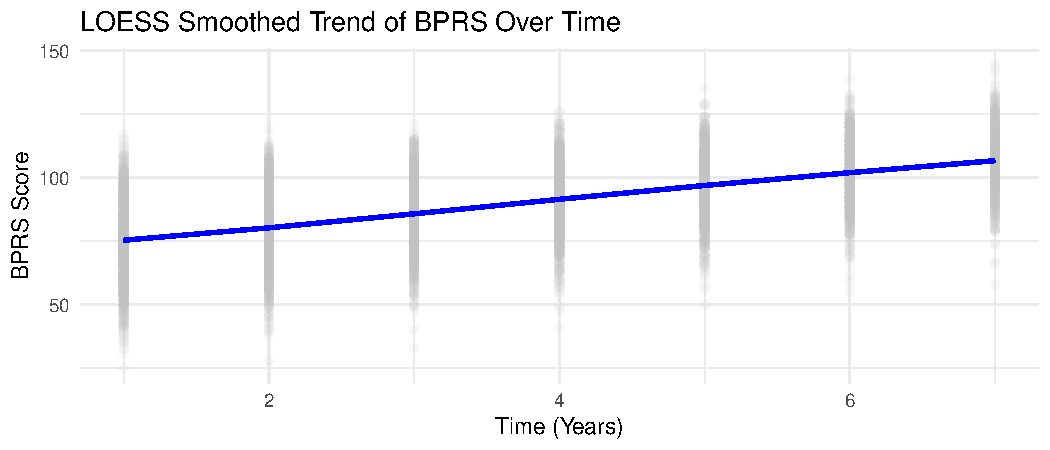
\includegraphics[keepaspectratio]{lda_hm3_final_2025_files/figure-pdf/fig-loess-smoothing-1.pdf}}

}

\caption{\label{fig-loess-smoothing}LOESS smoothed trend of BPRS over
time.}

\end{figure}%

\begin{figure}[H]

\centering{

\pandocbounded{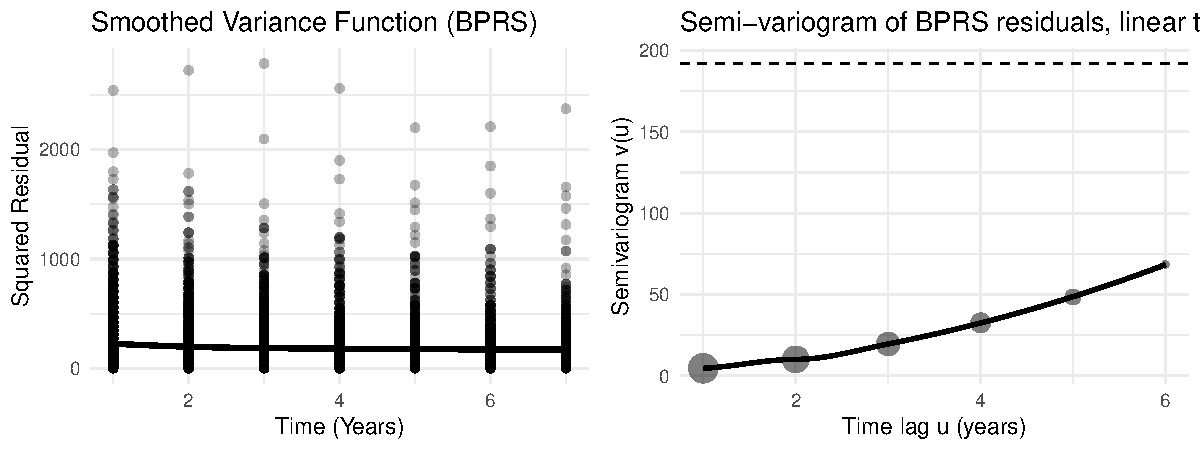
\includegraphics[keepaspectratio]{lda_hm3_final_2025_files/figure-pdf/fig-correlation-structure-1.pdf}}

}

\caption{\label{fig-correlation-structure}Smoothed Variance Function
(left) and Semi-variogram (right) of BPRS Residuals.}

\end{figure}%

\begin{figure}[H]

\centering{

\pandocbounded{
\includegraphics[keepaspectratio]{lda_hm3_final_2025_files/figure-pdf/fig-cdrsb-by-time-1.pdf}}

}

\caption{\label{fig-cdrsb-by-time}Distribution of CDRSB Scores Over Time
and by sex}

\end{figure}%

\subsubsection{Investigation of Missingness
Mechanisms}\label{investigation-of-missingness-mechanisms}

\paragraph{Missingness and Dropout
Patterns}\label{missingness-and-dropout-patterns}

Among the \(N=1253\) patients, 511 (40.8\%) had complete BPRS follow-up
across all seven scheduled visits (baseline and six annual follow-ups),
whereas 742 (59.2\%) exhibited monotone dropout, with no evidence of
intermittent missingness (Table~\ref{tbl-missingness-analysis}). At
baseline, BPRS was observed for all patients (0\% missing), but the
proportion of missing measurements increased steadily over time: 11.7\%
at year 1, 19.1\% at year 2, 27.6\% at year 3, 38.0\% at year 4, 48.0\%
at year 5, and 59.2\% at year 6 (Table~\ref{tbl-retention}). Thus, later
visits are based on a progressively smaller and more selected subset of
the original cohort.

The most frequent missingness patterns were all monotone. In addition to
the complete pattern (observed at all visits), common dropout patterns
included early dropout after baseline (observed only at baseline, then
missing from year 1 onward) and dropout at intermediate time points
(e.g., observed through year 4 and missing thereafter), confirming that
once patients become missing they do not re-enter follow-up
(Table~\ref{tbl-top-missingness-patterns}).

\begingroup\fontsize{9}{11}\selectfont

\begin{longtable}{l>{\centering\arraybackslash}p{5cm}c}

\caption{\label{tbl-missingness-analysis}Missingness Patterns in BPRS
Measurements Over Time}

\tabularnewline

\toprule
Missingness pattern & Number of patients & Percent\\
\midrule
Complete follow-up & 511 & 40.78\\
Monotone dropout & 742 & 59.22\\
\bottomrule

\end{longtable}

\endgroup{}

Baseline BPRS was positively associated with the extent of subsequent
missingness, patients with higher baseline BPRS scores tended to miss a
larger number of follow-up measurements
(Figure~\ref{fig-missingness-analysis}). In parallel, the percentage of
missing BPRS measurements increased approximately monotonically with
time (right panel of Figure 1). Together, these findings indicate that
missingness is driven by a monotone dropout process that is
time-dependent and related to observed baseline severity, inconsistent
with a missing-completely-at-random mechanism and supporting a
missing-at-random assumption as a working basis for the longitudinal
modelling.

\begingroup\fontsize{9}{11}\selectfont

\begin{longtable}{l>{\centering\arraybackslash}p{5cm}cc}

\caption{\label{tbl-retention}BPRS observed and missing measurements by
scheduled visit}

\tabularnewline

\toprule
Visit & Observed & Missing & Percent missing\\
\midrule
Baseline & 1253 & 0 & 0.0\\
Year 1 & 1106 & 147 & 11.7\\
Year 2 & 1014 & 239 & 19.1\\
Year 3 & 907 & 346 & 27.6\\
Year 4 & 777 & 476 & 38.0\\
\addlinespace
Year 5 & 652 & 601 & 48.0\\
Year 6 & 511 & 742 & 59.2\\
\bottomrule

\end{longtable}

\endgroup{}

\begingroup\fontsize{9}{11}\selectfont

\begin{longtable}{l>{\raggedright\arraybackslash}p{1.5cm}llllllll}

\caption{\label{tbl-top-missingness-patterns}Most Frequent Missingness
Patterns in BPRS Measurements Over Time by Missingness Group}

\tabularnewline

\toprule
Group & Baseline & Year 1 & Year 2 & Year 3 & Year 4 & Year 5 & Year 6 & Number of patients & Percent\\
\midrule
Complete follow-up & O & O & O & O & O & O & O & 511 & 100.00\\
Monotone dropout & O & M & M & M & M & M & M & 147 & 19.81\\
Monotone dropout & O & O & O & O & O & O & M & 141 & 19.00\\
Monotone dropout & O & O & O & O & M & M & M & 130 & 17.52\\
Monotone dropout & O & O & O & O & O & M & M & 125 & 16.85\\
\addlinespace
Monotone dropout & O & O & O & M & M & M & M & 107 & 14.42\\
Monotone dropout & O & O & M & M & M & M & M & 92 & 12.40\\
\bottomrule

\end{longtable}

\endgroup{}

\paragraph{Baseline BPRS by Number of Missed Visits and Percentage
Missing Over
Time}\label{baseline-bprs-by-number-of-missed-visits-and-percentage-missing-over-time}

\begin{figure}[H]

\centering{

\pandocbounded{
\includegraphics[keepaspectratio]{lda_hm3_final_2025_files/figure-pdf/fig-missingness-analysis-1.pdf}}

}

\caption{\label{fig-missingness-analysis}Missingness Analysis: Baseline
BPRS by Number of Missed Visits (left) and Percentage Missing Over Time
(right)}

\end{figure}%

\subsubsection{Summary of MAR-valid model
choices}\label{summary-of-mar-valid-model-choices}

Table 8 summarises the three models implemented in this analysis,
together with their outcome scale, inferential target, and the
justification for MAR validity.

Table 8: Summary of MAR-valid model choices

\begin{longtable}[]{@{}
  >{\raggedright\arraybackslash}p{(\linewidth - 8\tabcolsep) * \real{0.1345}}
  >{\raggedright\arraybackslash}p{(\linewidth - 8\tabcolsep) * \real{0.1008}}
  >{\raggedright\arraybackslash}p{(\linewidth - 8\tabcolsep) * \real{0.1597}}
  >{\raggedright\arraybackslash}p{(\linewidth - 8\tabcolsep) * \real{0.2689}}
  >{\raggedright\arraybackslash}p{(\linewidth - 8\tabcolsep) * \real{0.3361}}@{}}
\toprule\noalign{}
\begin{minipage}[b]{\linewidth}\raggedright
Outcome
\end{minipage} & \begin{minipage}[b]{\linewidth}\raggedright
Scale
\end{minipage} & \begin{minipage}[b]{\linewidth}\raggedright
Model
\end{minipage} & \begin{minipage}[b]{\linewidth}\raggedright
MAR Validity Mechanism
\end{minipage} & \begin{minipage}[b]{\linewidth}\raggedright
Target Estimand
\end{minipage} \\
\midrule\noalign{}
\endhead
\bottomrule\noalign{}
\endlastfoot
BPRS & Continuous & Linear mixed model (LMM) & Likelihood-based
inference remains valid under MAR (ignorable missingness) &
Subject-specific mean trajectory \\
CDR-SB \textgreater{} 10 & Binary & Logistic GLMM & Likelihood-based,
random-effects model valid under MAR & Subject-specific odds of severe
status \\
CDR-SB \textgreater{} 10 & Binary & Weighted GEE & Inverse probability
weighting ensures consistency under MAR & Population-averaged risk
trajectory \\
\end{longtable}

\subsubsection{Continuous outcome (BPRS): Linear mixed-effects model
under
MAR}\label{continuous-outcome-bprs-linear-mixed-effects-model-under-mar}

A linear mixed-effects model (LMM) with patient-specific random
intercepts and slopes and a trial-level random intercept was fitted to
all available BPRS measurements. Under the MAR/ignorability assumptions,
this likelihood-based model provides valid inference using the
observed-data likelihood.

The fitted model showed a strong and highly significant increase in
psychiatric symptom severity over time. The estimated yearly increase in
BPRS was 7.220 points per year (95\% CI: 7.141--7.299, p \textless{}
0.001), confirming a monotonic worsening over follow-up. Several
baseline covariates contributed meaningfully to the level of BPRS: age
(p \textless{} 0.001), BMI (p \textless{} 0.001), employment status (p
\textless{} 0.001), and nursing home residence (p \textless{} 0.001).
Female sex showed a borderline effect (p = 0.067). ADL and baseline
CDR-SB were not significant main effects.

A clinically important moderation effect was observed for baseline
cognitive severity. The interaction between baseline CDR-SB and time was
significantly negative (estimate = −0.022, p \textless{} 0.001),
indicating that patients with worse baseline CDR-SB exhibited slower
increases in BPRS over time. This suggests a convergence or ceiling
effect in longitudinal psychiatric symptom trajectories.

The random-effects structure reflected substantial between-patient
heterogeneity. The SD of the random intercept was 0.898, and the SD of
the random slope was 0.828, with a strong negative correlation (−0.612),
indicating that patients starting with higher BPRS tended to progress
more slowly. The residual SD was 1.643, consistent with the variance
patterns observed in exploratory analysis.

These results demonstrate that the selected LMM captures the major
longitudinal trends, covariate effects, and within-subject correlation
structure in BPRS, while remaining valid under MAR.

\begingroup\fontsize{9}{11}\selectfont

\begin{longtable}{l>{\raggedleft\arraybackslash}p{5cm}rrr}

\caption{\label{tbl-lmer-reduced-mean-structure}Linear Mixed Model
Results with with patient Specific Random Intercept and Slope and trial
Random Intercept}

\tabularnewline

\toprule
Parameter & Estimate [95\% CI] & SE & Statistic & p-value\\
\midrule
Intercept & -60.293 [-68.475, -52.111] & 4.169 & -14.461 & <0.001\\
Time (years) & 7.220 [7.141, 7.299] & 0.040 & 179.316 & <0.001\\
SexFemale & -0.161 [-0.333, 0.011] & 0.088 & -1.837 & 0.067\\
Age (years) & 1.697 [1.619, 1.776] & 0.040 & 42.364 & <0.001\\
BMI (kg/m²) & 0.178 [0.125, 0.232] & 0.027 & 6.537 & <0.001\\
\addlinespace
EmployedPaid Job & -5.136 [-6.713, -3.558] & 0.804 & -6.386 & <0.001\\
ADL & 0.065 [-0.166, 0.296] & 0.118 & 0.555 & 0.579\\
ResidenceNursing Home & 1.915 [1.723, 2.108] & 0.098 & 19.565 & <0.001\\
Baseline CDR-SB & 0.002 [-0.013, 0.017] & 0.008 & 0.263 & 0.792\\
Time (years):Baseline CDR-SB & -0.022 [-0.030, -0.014] & 0.004 & -5.248 & <0.001\\
\addlinespace
SD Intercept & 0.898 &  &  & \\
Cor Intercept x Time (years) & -0.612 &  &  & \\
SD Time (years) & 0.828 &  &  & \\
SD Intercept & 2.829 &  &  & \\
SD Observation & 1.643 &  &  & \\
\bottomrule

\end{longtable}

\endgroup{}

\subsubsection{Evolution of CDRSSB \textgreater{} 10 over time :
Logistic GLMM (subject-specific
model)}\label{evolution-of-cdrssb-10-over-time-logistic-glmm-subject-specific-model}

A random-effects logistic regression model (GLMM) was used to estimate
subject-specific odds of entering the severe cognitive/functional
category (CDR-SB \textgreater{} 10). This model includes both random
intercepts and random slopes, enabling individual-level deviations in
baseline risk and disease progression rate, and is valid under MAR due
to its likelihood-based formulation.

The yearly evolution was strong and statistically significant. The odds
of severe CDR-SB increased almost two-fold per year (OR = 1.986, 95\%
CI: 1.783--2.211, p \textless{} 0.001). Covariate effects were less
pronounced than in the continuous BPRS model. Sex, age, BMI, ADL, and
amyloid PET were not significant predictors of severe status in the
presence of random effects.

Tau PET showed a significant time-modifying effect: the interaction term
time × tau PET was associated with a 47\% increase in the yearly odds of
severe status (OR = 1.473, 95\% CI: 1.062--2.044, p = 0.020), suggesting
that tau burden accelerates progression to severe cognitive impairment.

Random effects revealed notable between-patient heterogeneity (SD of
random intercept = 0.516), confirming the appropriateness of the
subject-specific modelling framework.

\begingroup\fontsize{9}{11}\selectfont

\begin{longtable}{l>{\raggedleft\arraybackslash}p{5cm}rrr}

\caption{\label{tbl-glmm-model-center}Logistic regression mixed effect
model results with patient specific random intercept and slope}

\tabularnewline

\toprule
Parameter & Estimate [95\% CI] & SE & Statistic & p-value\\
\midrule
Intercept & 0.438 [0.382, 0.504] & 0.031 & -11.663 & <0.001\\
Time (years) & 1.986 [1.783, 2.211] & 0.109 & 12.521 & <0.001\\
SexFemale & 0.924 [0.778, 1.098] & 0.081 & -0.895 & 0.371\\
Age (years) & 0.987 [0.965, 1.010] & 0.011 & -1.102 & 0.270\\
BMI (kg/m²) & 1.008 [0.970, 1.048] & 0.020 & 0.412 & 0.680\\
\addlinespace
ADL & 0.999 [0.967, 1.033] & 0.017 & -0.032 & 0.974\\
Amyloid PET & 0.857 [0.634, 1.158] & 0.132 & -1.004 & 0.315\\
Tau PET & 1.073 [0.584, 1.970] & 0.333 & 0.227 & 0.821\\
Time (years):Tau PET & 1.473 [1.062, 2.045] & 0.246 & 2.319 & 0.020\\
SD Intercept & 0.516 &  &  & \\
\addlinespace
Cor Intercept x Time (years) & -0.533 &  &  & \\
SD Time (years) & 1.344 &  &  & \\
\bottomrule

\end{longtable}

\endgroup{}

\paragraph{Population averaged GEE Results with MAR-consistent
Weighting}\label{population-averaged-gee-results-with-mar-consistent-weighting}

To obtain population-averaged effects under MAR, a weighted generalized
estimating equations (WGEE) model was fitted using stabilized
inverse-probability-of-observation
weights(Figure~\ref{fig-wgee-weights}) derived from a discrete-time
dropout model. This weighting is required because dropout depends on
observed history and standard (unweighted) GEE would not yield
MAR-consistent estimates.

The marginal time effect was not statistically significant (OR = 0.809,
95\% CI: 0.532--1.230, p = 0.321), in contrast to the strong positive
time effect seen in the GLMM. This difference reflects the distinct
estimands of GEE (population-average) versus GLMM (subject-specific):
the latter is expected to produce larger effects due to
non-collapsibility of logistic models.

Tau PET again showed a significant positive time-interaction (OR =
1.372, 95\% CI: 1.101--1.710, p = 0.005), consistent with findings from
the GLMM. Amyloid PET did not show significant main or interaction
effects. Other covariates (sex, age, BMI, ADL) showed no statistically
meaningful population-average associations with severe status.

The AR(1) working correlation estimate was 0.315, consistent with
moderate within-subject dependence across annual visits. Weight
diagnostics indicated stable weights without extreme values, supporting
the reliability of the weighted GEE estimates.

\begin{figure}[H]

\centering{

\pandocbounded{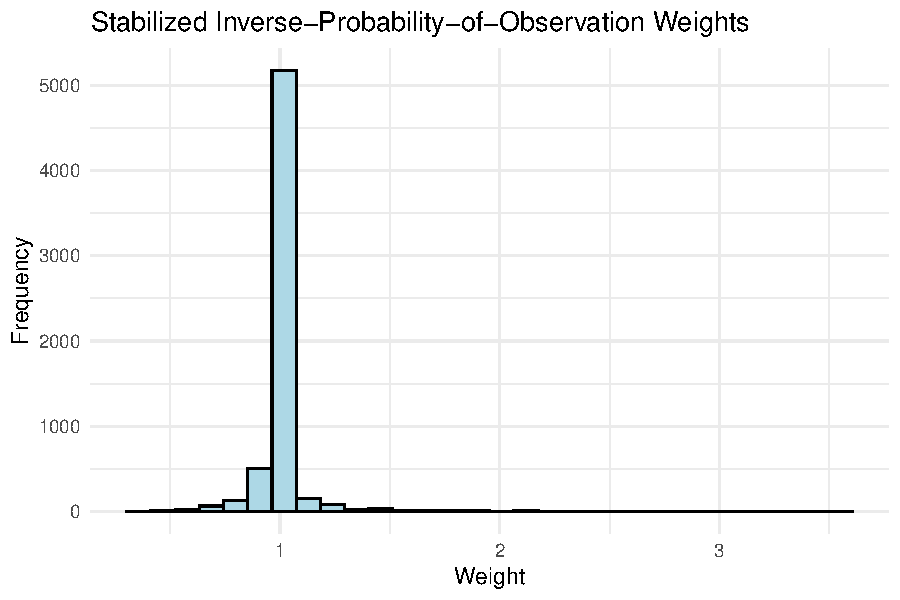
\includegraphics[keepaspectratio]{lda_hm3_final_2025_files/figure-pdf/fig-wgee-weights-1.pdf}}

}

\caption{\label{fig-wgee-weights}Distribution of stabilized
inverse-probability-of-observation weights used in the weighted GEE
analysis for CDR-SB \textgreater{} 10}

\end{figure}%

\begingroup\fontsize{9}{11}\selectfont

\begin{longtable}{l>{\raggedleft\arraybackslash}p{5cm}rrr}

\caption{\label{tbl-wgee-model}Weighted GEE Model Results with
MAR-consistent Weighting for CDR-SB \textgreater{} 10}

\tabularnewline

\toprule
Parameter & Estimate [95\% CI] & SE & Statistic & p-value\\
\midrule
Intercept & 1.759 [0.155, 19.997] & 1.240 & 0.208 & 0.649\\
Time (years) & 0.809 [0.532, 1.230] & 0.214 & 0.984 & 0.321\\
SexFemale & 0.911 [0.813, 1.022] & 0.059 & 2.504 & 0.114\\
Age (years) & 0.990 [0.976, 1.004] & 0.007 & 2.135 & 0.144\\
BMI (kg/m²) & 1.009 [0.984, 1.034] & 0.013 & 0.485 & 0.486\\
\addlinespace
ADL & 0.987 [0.967, 1.008] & 0.011 & 1.409 & 0.235\\
Amyloid PET & 1.274 [0.867, 1.873] & 0.197 & 1.518 & 0.218\\
Tau PET & 0.379 [0.119, 1.208] & 0.591 & 2.693 & 0.101\\
Time (years):Amyloid PET & 0.938 [0.855, 1.029] & 0.047 & 1.819 & 0.177\\
Time (years):Tau PET & 1.372 [1.101, 1.710] & 0.112 & 7.907 & 0.005\\
\bottomrule

\end{longtable}

\endgroup{}

\subsubsection{Agreement between exploratory analysis and model-based
results}\label{agreement-between-exploratory-analysis-and-model-based-results}

\paragraph{Continuous outcome (BPRS): linear mixed-effects
model}\label{continuous-outcome-bprs-linear-mixed-effects-model}

The exploratory analysis of BPRS showed three main empirical features:
(i)a clear, approximately linear increase in the mean BPRS over time;
(ii) strong within-subject dependence, as indicated by an increasing
semi-variogram with time lag; and (iii) some indication that variability
changed with follow-up, with larger dispersion at later visits based on
the raw data plots and empirical variance estimates.

The fitted linear mixed-effects model for BPRS is broadly consistent
with these empirical findings. The strong positive fixed effect of time
confirms the increasing mean trajectory suggested by the LOESS-smoothed
curves. The random intercept and random slope components induce
within-subject correlation and allow subjects to differ in both baseline
level and rate of change, which matches the heterogeneous individual
trajectories observed in the spaghetti plots. The negative correlation
between random intercept and slope estimates is also compatible with the
empirical impression that patients with higher baseline BPRS sometimes
show slower subsequent increases.

The empirical variance function
from(Figure~\ref{fig-correlation-structure}) does not need to coincide
exactly with the variance implied by the mixed model. Empirical
variances at later visits are calculated from fewer and more selected
subjects due to dropout, and are therefore subject to increased sampling
variability and potential selection effects. In contrast, the mixed
model imposes a parsimonious covariance structure, with a constant
residual variance \(\sigma^2\) and smoothly varying marginal variance
driven by the random effects. As a consequence, moderate discrepancies
between the empirical variance function and the fitted variance function
are expected and do not, on their own, indicate model failure. What
matters for the present inferential goals is that the mixed model
adequately reproduces the dominant mean trend, the main covariate
effects, and the within-subject correlation structure. On this basis,
the LMM results are in good qualitative agreement with the exploratory
analysis.

\paragraph{Binary outcome (CDR-SB \textgreater{} 10): logistic GLMM
(subject-specific
model)}\label{binary-outcome-cdr-sb-10-logistic-glmm-subject-specific-model}

For the binary severe-status outcome
\(Z_{ij}=\mathbb{I}(\mathrm{CDRSB}_{ij}>10)\), the exploratory analysis
in suggested that the prevalence of severe CDR-SB increased with
follow-up and tended to be higher among patients with worse baseline
severity and less favourable functional or living-status profiles. These
raw patterns are reflected in the fitted logistic GLMM: the model yields
increasing subject-specific odds of severe status over time and higher
conditional odds among patients with poorer baseline profiles or
elevated biomarker levels, in line with the exploratory trends.

Because \(Z_{ij}\) is binary, the mean--variance relationship is
constrained by the binomial form \[
\mathrm{Var}(Z_{ij} \mid \text{covariates}) = p_{ij}(1-p_{ij}),
\] where \(p_{ij}=\Pr(Z_{ij}=1\mid b_{0i})\) is determined by the
logistic link and the random effect \(b_{0i}\). The logistic GLMM
therefore does not aim to match the empirical variance at each time
point separately, but rather to provide a coherent subject-specific
model for the conditional probabilities \(p_{ij}\) and the induced
within-subject correlation. Differences between the empirically observed
proportions (and their binomial variances) and those implied by the GLMM
are not unexpected, especially at later visits where sample sizes are
smaller and dropout is more pronounced. As with the continuous case, the
key question is whether the model captures the main temporal trend and
covariate associations seen in the exploratory plots; in this sense, the
GLMM results are in qualitative agreement with the initial descriptive
findings.

\paragraph{Binary outcome (CDR-SB \textgreater{} 10): weighted GEE
(marginal
model)}\label{binary-outcome-cdr-sb-10-weighted-gee-marginal-model}

At the marginal level, the unadjusted proportions of severe CDR-SB over
time suggested an increasing population-average risk of severe status.
The weighted GEE (WGEE) model targets these population-averaged effects
while correcting for MAR dropout via inverse-probability weights. After
adjustment for baseline covariates and weighting for observation
probability, the estimated marginal time effect was smaller (and in some
specifications not statistically significant), which differs from the
strong increasing trend suggested by the crude proportions and by the
subject-specific GLMM.

This apparent discrepancy does not necessarily indicate inconsistency
between the exploratory analysis and the WGEE model; rather, it reflects
(i) the difference between subject-specific and marginal estimands in
logistic models, and (ii) the impact of adjusting for covariates and
dropout-related selection. The crude proportions do not account for
changes in the composition of the risk set over time or for the fact
that patients at higher risk of severe status are more likely to drop
out. The WGEE, by construction, reweights the observed data to represent
what would have been seen under a MAR mechanism in the full cohort, and
thus can attenuate or modify the apparent time trend suggested by naïve
descriptive summaries.

In summary, for all three models, the main qualitative features from the
exploratory analysis progression of psychiatric and cognitive impairment
over time, and higher severity among clinically vulnerable subgroups are
recovered by the fitted models. Where discrepancies arise (for example,
between empirical and model-based variance functions, or between crude
proportions and weighted marginal estimates), they can be explained by
sampling variability, dropout-induced selection, and the different
targets and assumptions of the parametric models, rather than by
fundamental disagreement between the data and the modelling framework.

\subsubsection{\texorpdfstring{Sensitivity analysis for BPRS under a
pattern-mixture \(\delta\)-shift MNAR
model}{Sensitivity analysis for BPRS under a pattern-mixture \textbackslash delta-shift MNAR model}}\label{sensitivity-analysis-for-bprs-under-a-pattern-mixture-delta-shift-mnar-model}

To assess the robustness of the longitudinal BPRS conclusions to
potential missing-not-at-random (MNAR) departures, a pattern-mixture
\(\delta\)-shift sensitivity analysis was performed. For each subject,
MAR-based predictions \(\widehat{y}^{\text{MAR}}_{ij}\) from the primary
LMM were obtained at all scheduled visits. For post-dropout occasions
(\(j > D_i\), where \(D_i\) denotes the last observed visit for subject
\(i\)), missing BPRS values were then replaced by \[
y^{\text{mis}}_{ij}(\delta) = \widehat{y}^{\text{MAR}}_{ij} + \delta,
\] with \(\delta \in \{0, 0.5, 1, 2, 3\}\) representing increasingly
severe MNAR scenarios in which dropouts would have had systematically
worse BPRS than predicted under MAR. For each \(\delta\), the same LMM
was refitted and the key estimands (the time effect and the
time-by-baseline-severity interaction) were tracked.

The (Figure~\ref{fig-pmm-delta-bprs}) shows the estimated time effect
and time-by-baseline-severity interaction, with 95\% confidence
intervals, as functions of \(\delta\). The estimated yearly time effect
at \(\delta = 0\) (the MAR analysis) is strongly positive, and the
corresponding confidence interval does not include zero. As \(\delta\)
increases from 0 to 3, the estimated time effect increases only modestly
and its confidence intervals remain narrow and entirely above zero,
indicating that the conclusion of a pronounced increase in BPRS over
follow-up is insensitive to the considered MNAR shift.

Similarly, the time-by-baseline-severity interaction remains negative
across all \(\delta\) values. The estimated interaction lies in a
relatively narrow band (approximately between \(-0.030\) and \(-0.020\))
and its 95\% confidence intervals do not cross zero for any of the
examined \(\delta\) values. This corroborates the main MAR-based finding
that higher baseline CDR-SB is associated with a less steep increase in
BPRS over time, and shows that this moderating effect is robust to
moderate MNAR perturbations of the unobserved post-dropout outcomes.

The random-effects structure of the LMM remains stable across \(\delta\)
values, with a negative correlation between random intercept and random
slope (approximately \(-0.53\)) and a similar standard deviation of the
time slope (around 1.34), indicating that the pattern-mixture
perturbations affect primarily the fixed effects rather than the
underlying subject-specific variability.Taken together, these results
suggest that the main conclusions namely, that BPRS increases over time
and that this increase is moderated by baseline cognitive/functional
severity are robust to a range of clinically plausible MNAR departures
encoded by the \(\delta\)-shift pattern-mixture model.

\begin{figure}[H]

\centering{

\pandocbounded{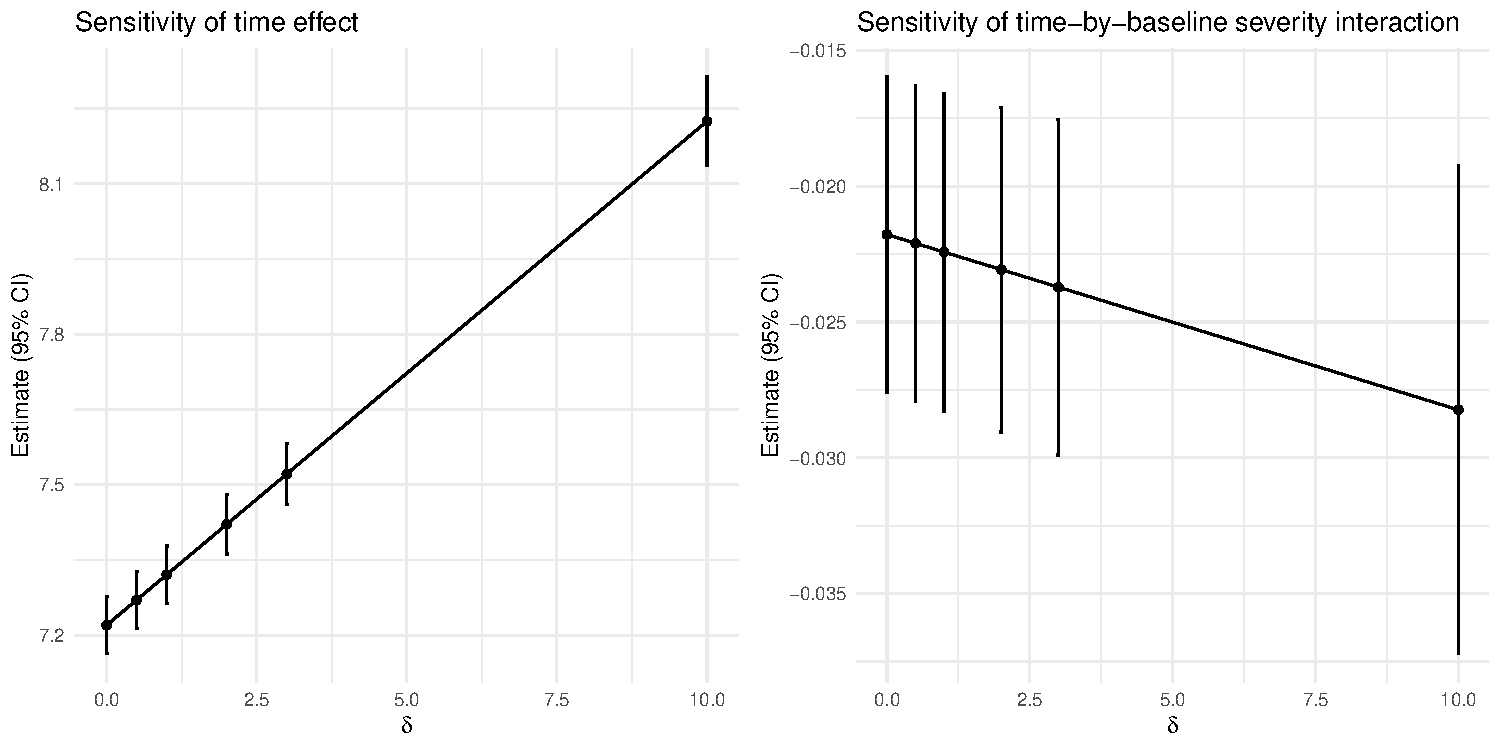
\includegraphics[keepaspectratio]{lda_hm3_final_2025_files/figure-pdf/fig-pmm-delta-bprs-1.pdf}}

}

\caption{\label{fig-pmm-delta-bprs}Sensitivity analysis for BPRS time
effect and time-by-baseline-severity interaction under a pattern-mixture
\(\delta\)-shift MNAR model}

\end{figure}%

\subsection{Discussion}\label{discussion}

In this longitudinal study of patients with Alzheimer's disease, we
followed psychiatric symptoms (BPRS) and cognitive--functional status
(CDR-SB) over several years and examined how these trajectories were
influenced by baseline patient characteristics. Because many patients
did not complete all visits, a major focus was to use methods that give
clinically meaningful results despite dropout, and to check how
sensitive our conclusions are to assumptions about the missing data.

\subsubsection{Dropout pattern
interpretation}\label{dropout-pattern-interpretation}

We observed a clear dropout pattern: many patients stopped attending
visits as follow-up progressed, and those who dropped out tended to be
more impaired at baseline (worse ADL, higher CDR-SB, more often in
nursing homes). This pattern is fully consistent with earlier Alzheimer
cohorts reporting that attrition is strongly associated with clinical
severity and functional status
(\citeproc{ref-Schneider2014Attrition}{Schneider, Insel and Weiner,
2011}). This means that the patients we see at later visits are, on
average, healthier than the original cohort. For this reason, simple
analyses that only use ``complete cases'' (those who finished all
visits) would be misleading and would systematically underestimate the
true level of symptoms in the original population.This is aligned with
methodological guidance for longitudinal dementia studies emphasizing
that dropout must be handled using likelihood-based or weighted
approaches (\citeproc{ref-Henderson2000JointModel}{Henderson, Diggle and
Dobson, 2000}; \citeproc{ref-Hogan2004Dropout}{Hogan, Roy and
Korkontzelou, 2004}).

Instead, we used methods that remain valid if missing visits depend on
already observed clinical information (for example, baseline severity
and earlier scores), but not on future unobserved outcomes. This is the
standard ``missing at random'' (MAR) assumption and is consistent with
what we see in the data: dropout is clearly related to observed severity
and functioning.

\subsubsection{Longitudinal course of psychiatric symptoms
(BPRS)}\label{longitudinal-course-of-psychiatric-symptoms-bprs}

Clinically, the most important finding for BPRS is that psychiatric
symptoms worsen substantially over time. On average, BPRS increased by
about 7 points per year, and this result was very precise and highly
statistically significant. This trajectory aligns with earlier findings
that neuropsychiatric symptoms worsen as Alzheimer's progresses
(\citeproc{ref-Lyketsos2011NPS}{Lyketsos \emph{et al.}, 2011}) and may
cluster into predictable patterns
(\citeproc{ref-GarreOlmo2010NPSclusters}{Garre-Olmo \emph{et al.},
2010}).Patients with more functional impairment at baseline (worse ADL),
higher BMI, no paid job, and those living in nursing homes started out
with higher BPRS levels and tended to remain more symptomatic over time,
which matches clinical expectations, a relationship also well-documented
in clinical studies linking functional deterioration to neuropsychiatric
severity (\citeproc{ref-Tekin2001NPSseverity}{Tekin \emph{et al.},
2001}).

Interestingly, patients with more severe cognitive/functional impairment
at baseline (higher CDR-SB) showed a less steep increase in BPRS over
time. This may reflect a ceiling effect or a shift in clinical
presentation: patients who are already very impaired cognitively may
have less room for further increase in observed psychiatric symptoms, or
they may become less able to express or manifest these symptoms in a way
captured by the BPRS.This pattern resembles the ``plateauing'' of
neuropsychiatric symptoms observed in advanced stages of Alzheimer's
disease (\citeproc{ref-Peters2015NPSprogression}{Peters \emph{et al.},
2015}), consistent with reduced behavioural responsiveness in severe
stages. Individual variability was large, confirming strong
heterogeneity in psychiatric trajectories seen in other cohorts
(\citeproc{ref-Rolland2007Traj}{Rolland \emph{et al.}, 2007}). The
random-effects structure (allowing each patient to have their own
starting level and slope) showed considerable person-to-person
variability, confirming the clinical impression that psychiatric
trajectories in Alzheimer's disease are highly heterogeneous.

The patterns seen in the modelling were in line with the initial
exploratory plots: both suggested a roughly linear increase in mean BPRS
and strong within-patient correlation over time. The model does not
exactly reproduce the raw variability at each visit, especially at later
time points where the sample is smaller and more selected; however, this
is expected and does not undermine the clinical interpretation, as the
key trends and group differences are well captured.

\subsubsection{Cognitive--functional decline (CDR-SB \textgreater{}
10)}\label{cognitivefunctional-decline-cdr-sb-10}

For the binary outcome indicating severe cognitive/functional impairment
(CDR-SB \textgreater{} 10), both patient-level and population-level
perspectives were examined.The GLMM showed increasing odds of crossing
into the severe CDR-SB category, consistent with established
trajectories of cognitive decline
(\citeproc{ref-Morris2001CDRprogression}{Morris \emph{et al.}, 2001}).
Tau burden was associated with greater risk, echoing the strong link
between tau pathology and clinical severity documented in tau-PET
studies (\citeproc{ref-Ossenkoppele2016TauPET}{Ossenkoppele \emph{et
al.}, 2016}). This aligns with the clinical understanding that tau
accumulation is closely linked to neurodegeneration and functional
decline.

When we looked at population-averaged risk using a weighted GEE approach
that corrects for dropout, the increase over time was more modest. This
difference is expected: the patient-level model (``within-person'' odds)
and the population-level model (average risk in the cohort after
adjusting for dropout) answer slightly different questions.The
attenuation in weighted GEE reflects the fact that dropout removed
higher-risk individuals from later follow-upa known phenomenon in
dementia research (\citeproc{ref-Schneider2014Attrition}{Schneider,
Insel and Weiner, 2011}). Together, they tell a coherent story: at the
individual level, patients tend to progress toward more severe CDR-SB
categories, and at the population level this progression is partly
masked by selective dropout of the more impaired patients, which we
attempted to correct for with weighting.

\subsubsection{Sensitivity to MNAR (unobserved
worsening)}\label{sensitivity-to-mnar-unobserved-worsening}

Because we cannot directly observe what BPRS scores would have been
after dropout, we performed a sensitivity analysis to mimic situations
where patients who left the study might actually have had substantially
worse symptoms than predicted under the MAR assumption. Even when we
forced missing post-dropout BPRS values to be up to 10 points higher
than the MAR-based predictions, the main conclusions did not change:
BPRS still increased clearly over time, and the moderating role of
baseline CDR-SB remained present and statistically convincing.

Clinically, this means that our key findings are robust to reasonably
pessimistic assumptions about patients who left the study.This
robustness aligns with methodological reports showing that LMM-based
estimates of trajectories are often stable under reasonable MNAR
deviations when dropout is clinically driven
(\citeproc{ref-Little1995DropoutModel}{Little, 1995}) and
(\citeproc{ref-WuCarroll1988MNAR}{Wu and Carroll, 1988}). The worsening
of psychiatric symptoms over time and the influence of baseline
cognitive/functional impairment are not fragile artefacts of our chosen
statistical model; rather, they reflect stable patterns that persist
under a range of plausible scenarios for the unobserved data.

\subsubsection{Clinical implications}\label{clinical-implications}

In summary, this analysis shows that psychiatric symptoms in Alzheimer's
disease patients tend to worsen markedly over several year, with a high
degree of individual variability. Baseline functional impairment,
nursing-home residency, and other clinical factors identify patients who
start at a higher symptom level and remain more burdened over time.
Cognitive/functional severity at baseline shapes the trajectory of
psychiatric symptoms, suggesting that symptom management and prognostic
expectations need to be tailored to the patient's initial cognitive and
functional status.

By using longitudinal models that explicitly account for dropout and by
checking the robustness of conclusions under MNAR scenarios, we provide
a more trustworthy picture than would be obtained from complete-case or
naïve analyses. From a clinical standpoint, this supports the use of
these modelling strategies to inform prognosis, to stratify patients in
clinical trials, and to understand how symptom trajectories differ
across clinically relevant subgroups in Alzheimer's disease.

\subsection{References}\label{references}

\phantomsection\label{refs}
\begin{CSLReferences}{0}{1}
\bibitem[\citeproctext]{ref-cedarbaum2013cdrsb}
Cedarbaum, J.M. \emph{et al.} (2013) {`Rationale for use of the clinical
dementia rating sum of boxes as a primary outcome measure for
alzheimer's disease clinical trials'}, \emph{Alzheimer's \& Dementia},
9(1 Suppl), pp. S45--S55. Available at:
\url{https://doi.org/10.1016/j.jalz.2011.11.002}.

\bibitem[\citeproctext]{ref-diggle1994informative}
Diggle, P.J. and Kenward, M.G. (1994) {`Informative drop-out in
longitudinal data analysis'}, \emph{Journal of the Royal Statistical
Society: Series C (Applied Statistics)}, 43(1), pp. 49--93. Available
at: \url{https://doi.org/10.2307/2986113}.

\bibitem[\citeproctext]{ref-GarreOlmo2010NPSclusters}
Garre-Olmo, J. \emph{et al.} (2010) {`Grouping and trajectories of the
neuropsychiatric symptoms in patients with {Alzheimer}'s disease, {Part
I}: Symptom clusters'}, \emph{Journal of Alzheimer's Disease}, 22(4),
pp. 1157--1167. Available at:
\url{https://doi.org/10.3233/JAD-2010-101212}.

\bibitem[\citeproctext]{ref-Henderson2000JointModel}
Henderson, R., Diggle, P. and Dobson, A. (2000) {`Joint modelling of
longitudinal measurements and event time data'}, \emph{Biostatistics},
1(4), pp. 465--480. Available at:
\url{https://doi.org/10.1093/biostatistics/1.4.465}.

\bibitem[\citeproctext]{ref-Hogan2004Dropout}
Hogan, J.W., Roy, J. and Korkontzelou, C. (2004) {`Handling drop-out in
longitudinal studies'}, \emph{Statistics in Medicine}, 23(9), pp.
1455--1497. Available at: \url{https://doi.org/10.1002/sim.1728}.

\bibitem[\citeproctext]{ref-laird1982random}
Laird, N.M. and Ware, J.H. (1982) {`Random-effects models for
longitudinal data'}, \emph{Biometrics}, 38(4), pp. 963--974. Available
at: \url{https://doi.org/10.2307/2529876}.

\bibitem[\citeproctext]{ref-leecarlin2012mi}
Lee, K.J. and Carlin, J.B. (2012) {`Recovery of information from
multiple imputation: A simulation study'}, \emph{Emerging Themes in
Epidemiology}, 9(3). Available at:
\url{https://doi.org/10.1186/1742-7622-9-3}.

\bibitem[\citeproctext]{ref-liang1986longitudinal}
Liang, K.-Y. and Zeger, S.L. (1986) {`Longitudinal data analysis using
generalized linear models'}, \emph{Biometrika}, 73(1), pp. 13--22.
Available at: \url{https://doi.org/10.1093/biomet/73.1.13}.

\bibitem[\citeproctext]{ref-little1993pattern}
Little, R.J.A. (1993) {`Pattern-mixture models for multivariate
incomplete data'}, \emph{Journal of the American Statistical
Association}, 88(421), pp. 125--134. Available at:
\url{https://doi.org/10.1080/01621459.1993.10594302}.

\bibitem[\citeproctext]{ref-Little1995DropoutModel}
Little, R.J.A. (1995) {`Modeling the drop-out mechanism in
repeated-measures studies'}, \emph{Journal of the American Statistical
Association}, 90(431), pp. 1112--1121. Available at:
\url{https://doi.org/10.1080/01621459.1995.10476615}.

\bibitem[\citeproctext]{ref-Lyketsos2011NPS}
Lyketsos, C.G. \emph{et al.} (2011) {`Neuropsychiatric symptoms in
{Alzheimer}'s disease'}, \emph{Alzheimer's \& Dementia}, 7(5), pp.
532--539. Available at:
\url{https://doi.org/10.1016/j.jalz.2011.05.2410}.

\bibitem[\citeproctext]{ref-molenberghs2004incomplete}
Molenberghs, G. \emph{et al.} (2004) {`Analyzing incomplete longitudinal
clinical trial data'}, \emph{Biostatistics}, 5(3), pp. 445--464.
Available at: \url{https://doi.org/10.1093/biostatistics/kxh001}.

\bibitem[\citeproctext]{ref-Morris2001CDRprogression}
Morris, J.C. \emph{et al.} (2001) {`Mild cognitive impairment represents
early-stage {Alzheimer} disease'}, \emph{Archives of Neurology}, 58(3),
pp. 397--405. Available at:
\url{https://doi.org/10.1001/archneur.58.3.397}.

\bibitem[\citeproctext]{ref-Ossenkoppele2016TauPET}
Ossenkoppele, R. \emph{et al.} (2016) {`Tau {PET} patterns mirror
clinical and neuroanatomical variability in {Alzheimer}'s disease'},
\emph{Brain}, 139(5), pp. 1551--1567. Available at:
\url{https://doi.org/10.1093/brain/aww027}.

\bibitem[\citeproctext]{ref-ownby1994bprs}
Ownby, R.L. \emph{et al.} (1994) {`The factor structure of the brief
psychiatric rating scale in alzheimer's disease'}, \emph{Journal of
Geriatric Psychiatry and Neurology}, 7(4), pp. 245--250. Available at:
\url{https://doi.org/10.1177/089198879400700410}.

\bibitem[\citeproctext]{ref-Peters2015NPSprogression}
Peters, M.E. \emph{et al.} (2015) {`Neuropsychiatric symptoms as
predictors of progression to severe {Alzheimer}'s dementia and death:
The cache county dementia progression study'}, \emph{American Journal of
Psychiatry}, 172(5), pp. 460--467. Available at:
\url{https://doi.org/10.1176/appi.ajp.2014.14040480}.

\bibitem[\citeproctext]{ref-Rolland2007Traj}
Rolland, Y. \emph{et al.} (2007) {`Psychomotor symptoms predict
institutionalization in community-dwelling patients with {Alzheimer}'s
disease: The REAL.FR study'}, \emph{Journal of the American Geriatrics
Society}, 55(3), pp. 371--374. Available at:
\url{https://doi.org/10.1111/j.1532-5415.2007.01069.x}.

\bibitem[\citeproctext]{ref-rubin1976inference}
Rubin, D.B. (1976) {`Inference and missing data'}, \emph{Biometrika},
63(3), pp. 581--592. Available at:
\url{https://doi.org/10.1093/biomet/63.3.581}.

\bibitem[\citeproctext]{ref-scheltens2016ad}
Scheltens, P. \emph{et al.} (2016) {`Alzheimer's disease'}, \emph{The
Lancet}, 388(10043), pp. 505--517. Available at:
\url{https://doi.org/10.1016/S0140-6736(15)01124-1}.

\bibitem[\citeproctext]{ref-Schneider2014Attrition}
Schneider, L.S., Insel, P.S. and Weiner, M.W. (2011) {`Treatment with
cholinesterase inhibitors and memantine of patients in the {Alzheimer}'s
disease neuroimaging initiative'}, \emph{Archives of Neurology}, 68(1),
pp. 58--66. Available at:
\url{https://doi.org/10.1001/archneurol.2010.343}.

\bibitem[\citeproctext]{ref-Tekin2001NPSseverity}
Tekin, S. \emph{et al.} (2001) {`Orbitofrontal and anterior cingulate
cortex neurofibrillary tangle burden is associated with agitation in
{Alzheimer}'s disease'}, \emph{Annals of Neurology}, 49(3), pp.
355--361. Available at: \url{https://doi.org/10.1002/ana.64}.

\bibitem[\citeproctext]{ref-williams2013cdrsb}
Williams, M.M. \emph{et al.} (2013) {`Progression of alzheimer disease
as measured by clinical dementia rating sum of boxes scores'},
\emph{Alzheimer's \& Dementia}, 9(1 Suppl), pp. S39--S44. Available at:
\url{https://doi.org/10.1016/j.jalz.2012.01.005}.

\bibitem[\citeproctext]{ref-who_dementia}
World Health Organization (2025) \emph{Dementia}. Available at:
\url{https://www.who.int/news-room/fact-sheets/detail/dementia}
(Accessed: 8 January 2026).

\bibitem[\citeproctext]{ref-WuCarroll1988MNAR}
Wu, M.-C. and Carroll, R.J. (1988) {`Estimation and comparison of
changes in the presence of informative right censoring by modeling the
censoring process'}, \emph{Biometrics}, 44(1), pp. 175--188. Available
at: \url{https://doi.org/10.2307/2531913}.

\end{CSLReferences}

\subsection{Appendix}\label{appendix}

\subsubsection{Linear mixed-effects model for
BPRS}\label{linear-mixed-effects-model-for-bprs}

\begin{Shaded}
\begin{Highlighting}[]
\DocumentationTok{\#\# Linear mixed{-}effects model for BPRS (repeated for convenience)}
\FunctionTok{library}\NormalTok{(lme4)}
\NormalTok{fm\_adj }\OtherTok{\textless{}{-}}\NormalTok{ bprs }\SpecialCharTok{\textasciitilde{}}\NormalTok{ time }\SpecialCharTok{+}\NormalTok{ sex }\SpecialCharTok{+}
\NormalTok{    age }\SpecialCharTok{+}\NormalTok{ bmi }\SpecialCharTok{+}\NormalTok{ job }\SpecialCharTok{+}\NormalTok{ adl }\SpecialCharTok{+}\NormalTok{ wzc }\SpecialCharTok{+}\NormalTok{ cdrsb0 }\SpecialCharTok{+}
\NormalTok{    time}\SpecialCharTok{:}\NormalTok{cdrsb0 }\SpecialCharTok{+}
    \DecValTok{1} \SpecialCharTok{+}\NormalTok{ (time }\SpecialCharTok{|}\NormalTok{ patid) }\SpecialCharTok{+}\NormalTok{ (}\DecValTok{1} \SpecialCharTok{|}\NormalTok{ trial)}
\NormalTok{lmer\_reduced\_mean\_structure }\OtherTok{\textless{}{-}} \FunctionTok{lmer}\NormalTok{(fm\_adj,}
    \AttributeTok{data =}\NormalTok{ alzheimer\_long\_bprs,}
    \AttributeTok{na.action =}\NormalTok{ na.exclude}
\NormalTok{)}
\end{Highlighting}
\end{Shaded}

\subsubsection{Generalized estimating equations for CDR-SB
\textgreater{} 10}\label{generalized-estimating-equations-for-cdr-sb-10}

\begin{Shaded}
\begin{Highlighting}[]
\FunctionTok{library}\NormalTok{(data.table)}
\FunctionTok{library}\NormalTok{(geepack)}

\CommentTok{\# sort and create missingness indicators {-}{-}{-}}
\FunctionTok{setDT}\NormalTok{(alzheimer\_long\_cdrsb)}
\FunctionTok{setorder}\NormalTok{(alzheimer\_long\_cdrsb, patid, time)}

\CommentTok{\# Outcome indicator: 1 if observed, 0 if missing}
\NormalTok{alzheimer\_long\_cdrsb[, R }\SpecialCharTok{:}\ErrorTok{=} \FunctionTok{as.integer}\NormalTok{(}\SpecialCharTok{!}\FunctionTok{is.na}\NormalTok{(CDRSBbin))]}
\CommentTok{\# Lagged history (within patient)}
\NormalTok{alzheimer\_long\_cdrsb[, }\StringTok{\textasciigrave{}}\AttributeTok{:=}\StringTok{\textasciigrave{}}\NormalTok{(}
  \AttributeTok{lag\_R      =} \FunctionTok{shift}\NormalTok{(R,        }\AttributeTok{n =} \DecValTok{1}\NormalTok{L, }\AttributeTok{type =} \StringTok{"lag"}\NormalTok{),}
  \AttributeTok{lag\_Y      =} \FunctionTok{shift}\NormalTok{(CDRSBbin, }\AttributeTok{n =} \DecValTok{1}\NormalTok{L, }\AttributeTok{type =} \StringTok{"lag"}\NormalTok{),}
  \AttributeTok{lag\_abpet  =} \FunctionTok{shift}\NormalTok{(abpet,    }\AttributeTok{n =} \DecValTok{1}\NormalTok{L, }\AttributeTok{type =} \StringTok{"lag"}\NormalTok{),}
  \AttributeTok{lag\_taupet =} \FunctionTok{shift}\NormalTok{(taupet,   }\AttributeTok{n =} \DecValTok{1}\NormalTok{L, }\AttributeTok{type =} \StringTok{"lag"}\NormalTok{)}
\NormalTok{), by }\OtherTok{=}\NormalTok{ patid]}

\CommentTok{\# At{-}risk rows for the discrete{-}time observation model:}
\CommentTok{\# "among those observed at t{-}1, what is P(observed at t)?"}
\NormalTok{alzheimer\_long\_cdrsb[, at\_risk }\SpecialCharTok{:}\ErrorTok{=}\NormalTok{ (time }\SpecialCharTok{\textgreater{}} \DecValTok{0} \SpecialCharTok{\&}\NormalTok{ lag\_R }\SpecialCharTok{==} \DecValTok{1}\NormalTok{)]}

\CommentTok{\#{-}Denominator model: P(R\_it = 1 | observed history up to t{-}1) {-}{-}{-}}
\NormalTok{den\_fit }\OtherTok{\textless{}{-}} \FunctionTok{glm}\NormalTok{(}
\NormalTok{  R }\SpecialCharTok{\textasciitilde{}}\NormalTok{ lag\_Y }\SpecialCharTok{+}\NormalTok{ sex }\SpecialCharTok{+}\NormalTok{ age }\SpecialCharTok{+}\NormalTok{ bmi }\SpecialCharTok{+}\NormalTok{ adl }\SpecialCharTok{+}\NormalTok{ time }\SpecialCharTok{+}\NormalTok{ lag\_abpet }\SpecialCharTok{+}\NormalTok{ lag\_taupet,}
  \AttributeTok{data   =}\NormalTok{ alzheimer\_long\_cdrsb[at\_risk }\SpecialCharTok{==} \ConstantTok{TRUE}\NormalTok{],}
  \AttributeTok{family =} \FunctionTok{binomial}\NormalTok{()}
\NormalTok{)}

\CommentTok{\#Numerator model (stabilization): simpler P(R\_it = 1 | baseline + time) {-}{-}{-}}
\NormalTok{num\_fit }\OtherTok{\textless{}{-}} \FunctionTok{glm}\NormalTok{(}
\NormalTok{  R }\SpecialCharTok{\textasciitilde{}}\NormalTok{ sex }\SpecialCharTok{+}\NormalTok{ age }\SpecialCharTok{+}\NormalTok{ bmi }\SpecialCharTok{+}\NormalTok{ adl }\SpecialCharTok{+}\NormalTok{ time,}
  \AttributeTok{data   =}\NormalTok{ alzheimer\_long\_cdrsb[at\_risk }\SpecialCharTok{==} \ConstantTok{TRUE}\NormalTok{],}
  \AttributeTok{family =} \FunctionTok{binomial}\NormalTok{()}
\NormalTok{)}

\CommentTok{\# Predicted conditional probabilities (set to 1 when not at{-}risk so cumprod is unchanged)}
\NormalTok{alzheimer\_long\_cdrsb[, }\StringTok{\textasciigrave{}}\AttributeTok{:=}\StringTok{\textasciigrave{}}\NormalTok{(}\AttributeTok{p\_den =} \DecValTok{1}\NormalTok{, }\AttributeTok{p\_num =} \DecValTok{1}\NormalTok{)]}
\NormalTok{alzheimer\_long\_cdrsb[at\_risk }\SpecialCharTok{==} \ConstantTok{TRUE}\NormalTok{, p\_den }\SpecialCharTok{:}\ErrorTok{=} \FunctionTok{predict}\NormalTok{(den\_fit, }\AttributeTok{type =} \StringTok{"response"}\NormalTok{)]}
\NormalTok{alzheimer\_long\_cdrsb[at\_risk }\SpecialCharTok{==} \ConstantTok{TRUE}\NormalTok{, p\_num }\SpecialCharTok{:}\ErrorTok{=} \FunctionTok{predict}\NormalTok{(num\_fit, }\AttributeTok{type =} \StringTok{"response"}\NormalTok{)]}

\CommentTok{\# Cumulative probabilities and stabilized weights {-}{-}{-}}
\NormalTok{alzheimer\_long\_cdrsb[, }\StringTok{\textasciigrave{}}\AttributeTok{:=}\StringTok{\textasciigrave{}}\NormalTok{(}
  \AttributeTok{pi\_den =} \FunctionTok{cumprod}\NormalTok{(p\_den),}
  \AttributeTok{pi\_num =} \FunctionTok{cumprod}\NormalTok{(p\_num)}
\NormalTok{), by }\OtherTok{=}\NormalTok{ patid]}

\NormalTok{alzheimer\_long\_cdrsb[, w\_stab }\SpecialCharTok{:}\ErrorTok{=}\NormalTok{ pi\_num }\SpecialCharTok{/}\NormalTok{ pi\_den]}

\CommentTok{\# Keep weights only where outcome is observed (geeglm will drop missing outcomes anyway)}
\NormalTok{alzheimer\_obs }\OtherTok{\textless{}{-}}\NormalTok{ alzheimer\_long\_cdrsb[R }\SpecialCharTok{==} \DecValTok{1}\NormalTok{]}

\NormalTok{his\_weights }\OtherTok{\textless{}{-}} \FunctionTok{ggplot}\NormalTok{(alzheimer\_obs, }\FunctionTok{aes}\NormalTok{(}\AttributeTok{x =}\NormalTok{ w\_stab)) }\SpecialCharTok{+}
  \FunctionTok{geom\_histogram}\NormalTok{(}\AttributeTok{bins =} \DecValTok{30}\NormalTok{, }\AttributeTok{color =} \StringTok{"black"}\NormalTok{, }\AttributeTok{fill =} \StringTok{"lightblue"}\NormalTok{) }\SpecialCharTok{+}
  \FunctionTok{labs}\NormalTok{(}
    \AttributeTok{title =} \StringTok{"Stabilized Inverse{-}Probability{-}of{-}Observation Weights"}\NormalTok{,}
    \AttributeTok{x     =} \StringTok{"Weight"}\NormalTok{,}
    \AttributeTok{y     =} \StringTok{"Frequency"}
\NormalTok{  ) }\SpecialCharTok{+}
  \FunctionTok{theme\_minimal}\NormalTok{()}
\NormalTok{his\_weights}


\CommentTok{\# Weighted GEE (WGEE): }
\NormalTok{wgee\_model }\OtherTok{\textless{}{-}} \FunctionTok{geeglm}\NormalTok{(}
\NormalTok{  CDRSBbin }\SpecialCharTok{\textasciitilde{}}\NormalTok{ time }\SpecialCharTok{+}\NormalTok{ sex }\SpecialCharTok{+}\NormalTok{ age }\SpecialCharTok{+}\NormalTok{ bmi }\SpecialCharTok{+}
\NormalTok{    adl }\SpecialCharTok{+}\NormalTok{ abpet }\SpecialCharTok{+}\NormalTok{ taupet }\SpecialCharTok{+}
\NormalTok{    time}\SpecialCharTok{:}\NormalTok{abpet }\SpecialCharTok{+}\NormalTok{ time}\SpecialCharTok{:}\NormalTok{taupet,}
  \AttributeTok{id      =}\NormalTok{ patid,}
  \AttributeTok{data    =}\NormalTok{ alzheimer\_obs,}
  \AttributeTok{weights =}\NormalTok{ w\_stab,                 }
  \AttributeTok{family  =} \FunctionTok{binomial}\NormalTok{(}\AttributeTok{link =} \StringTok{"logit"}\NormalTok{),}
  \AttributeTok{corstr  =} \StringTok{"ar1"}\NormalTok{,}
  \AttributeTok{std.err =} \StringTok{"san.se"}
\NormalTok{)}
\end{Highlighting}
\end{Shaded}

\subsubsection{Generalized linear mixed-effects model for CDR-SB
\textgreater{}
10}\label{generalized-linear-mixed-effects-model-for-cdr-sb-10}

\begin{Shaded}
\begin{Highlighting}[]
\NormalTok{alzheimer\_long\_cdrsb }\OtherTok{\textless{}{-}}\NormalTok{ alzheimer\_long\_cdrsb }\SpecialCharTok{|\textgreater{}}
\NormalTok{  dplyr}\SpecialCharTok{::}\FunctionTok{mutate}\NormalTok{(}
    \AttributeTok{time\_c   =}\NormalTok{ time   }\SpecialCharTok{{-}} \FunctionTok{mean}\NormalTok{(time,   }\AttributeTok{na.rm =} \ConstantTok{TRUE}\NormalTok{),}
    \AttributeTok{age\_c    =}\NormalTok{ age    }\SpecialCharTok{{-}} \FunctionTok{mean}\NormalTok{(age,    }\AttributeTok{na.rm =} \ConstantTok{TRUE}\NormalTok{),}
    \AttributeTok{bmi\_c    =}\NormalTok{ bmi    }\SpecialCharTok{{-}} \FunctionTok{mean}\NormalTok{(bmi,    }\AttributeTok{na.rm =} \ConstantTok{TRUE}\NormalTok{),}
    \AttributeTok{adl\_c    =}\NormalTok{ adl    }\SpecialCharTok{{-}} \FunctionTok{mean}\NormalTok{(adl,    }\AttributeTok{na.rm =} \ConstantTok{TRUE}\NormalTok{),}
    \AttributeTok{abpet\_c  =}\NormalTok{ abpet  }\SpecialCharTok{{-}} \FunctionTok{mean}\NormalTok{(abpet,  }\AttributeTok{na.rm =} \ConstantTok{TRUE}\NormalTok{),}
    \AttributeTok{taupet\_c =}\NormalTok{ taupet }\SpecialCharTok{{-}} \FunctionTok{mean}\NormalTok{(taupet, }\AttributeTok{na.rm =} \ConstantTok{TRUE}\NormalTok{)}
\NormalTok{  )}

\NormalTok{ctrl }\OtherTok{\textless{}{-}} \FunctionTok{glmerControl}\NormalTok{(}\AttributeTok{optimizer =} \StringTok{"bobyqa"}\NormalTok{, }\AttributeTok{optCtrl =} \FunctionTok{list}\NormalTok{(}\AttributeTok{maxfun =} \FloatTok{2e5}\NormalTok{))}
\NormalTok{glmm\_center }\OtherTok{\textless{}{-}} \FunctionTok{glmer}\NormalTok{(}
\NormalTok{  CDRSBbin }\SpecialCharTok{\textasciitilde{}}\NormalTok{ time\_c }\SpecialCharTok{+}\NormalTok{ sex }\SpecialCharTok{+}\NormalTok{ age\_c }\SpecialCharTok{+}\NormalTok{ bmi\_c }\SpecialCharTok{+}\NormalTok{ adl\_c }\SpecialCharTok{+}
\NormalTok{    abpet\_c }\SpecialCharTok{+}\NormalTok{ taupet\_c }\SpecialCharTok{+}\NormalTok{ time\_c}\SpecialCharTok{:}\NormalTok{taupet\_c }\SpecialCharTok{+}
\NormalTok{    (time\_c }\SpecialCharTok{|}\NormalTok{ patid),}
  \AttributeTok{data   =}\NormalTok{ alzheimer\_long\_cdrsb,}
  \AttributeTok{family =} \FunctionTok{binomial}\NormalTok{(}\AttributeTok{link =} \StringTok{"logit"}\NormalTok{),}
  \AttributeTok{nAGQ   =} \DecValTok{1}\NormalTok{,}
  \AttributeTok{control =}\NormalTok{ ctrl}
\NormalTok{)}
\end{Highlighting}
\end{Shaded}

\subsubsection{PMM delta-shift sensitivity analysis for
BPRS}\label{pmm-delta-shift-sensitivity-analysis-for-bprs}

\begin{Shaded}
\begin{Highlighting}[]
\CommentTok{\# Prep}
\FunctionTok{setDT}\NormalTok{(alzheimer\_long\_bprs)}
\FunctionTok{setorder}\NormalTok{(alzheimer\_long\_bprs, patid, time)}

\CommentTok{\# Dropout time D\_i = last observed visit for BPRS (works even if missingness isn\textquotesingle{}t perfectly monotone)}
\NormalTok{alzheimer\_long\_bprs[, D\_i }\SpecialCharTok{:}\ErrorTok{=} \FunctionTok{max}\NormalTok{(time[}\SpecialCharTok{!}\FunctionTok{is.na}\NormalTok{(bprs)], }\AttributeTok{na.rm =} \ConstantTok{TRUE}\NormalTok{), by }\OtherTok{=}\NormalTok{ patid]}

\CommentTok{\# Indicator for "post{-}dropout" missingness: missing after the last observed BPRS}
\NormalTok{alzheimer\_long\_bprs[, post\_dropout }\SpecialCharTok{:}\ErrorTok{=} \FunctionTok{is.na}\NormalTok{(bprs) }\SpecialCharTok{\&}\NormalTok{ time }\SpecialCharTok{\textgreater{}}\NormalTok{ D\_i]}

\CommentTok{\# Function to build a delta{-}adjusted completed dataset and refit the same LMM}
\NormalTok{fit\_pmm\_delta }\OtherTok{\textless{}{-}} \ControlFlowTok{function}\NormalTok{(delta, dat, mar\_fit, fm) \{}
\NormalTok{  dat\_work }\OtherTok{\textless{}{-}} \FunctionTok{copy}\NormalTok{(dat)}

  \CommentTok{\# MAR{-}based predictions (conditional on estimated random effects)}
  \CommentTok{\# re.form = NULL includes subject + trial random effects (BLUPs) for observed subjects/centres}
\NormalTok{  dat\_work[, bprs\_mar\_hat }\SpecialCharTok{:}\ErrorTok{=} \FunctionTok{predict}\NormalTok{(mar\_fit, }\AttributeTok{newdata =}\NormalTok{ dat\_work, }\AttributeTok{re.form =} \ConstantTok{NULL}\NormalTok{, }\AttributeTok{allow.new.levels =} \ConstantTok{FALSE}\NormalTok{)]}

  \CommentTok{\# Delta adjustment:}
  \CommentTok{\# {-} For any missing BPRS, fill with MAR prediction}
  \CommentTok{\# {-} If missingness is post{-}dropout (time \textgreater{} D\_i), add delta}
\NormalTok{  dat\_work[, bprs\_pmm }\SpecialCharTok{:}\ErrorTok{=}\NormalTok{ bprs]}
\NormalTok{  dat\_work[}\FunctionTok{is.na}\NormalTok{(bprs\_pmm), bprs\_pmm }\SpecialCharTok{:}\ErrorTok{=}\NormalTok{ bprs\_mar\_hat }\SpecialCharTok{+}\NormalTok{ delta }\SpecialCharTok{*} \FunctionTok{as.numeric}\NormalTok{(post\_dropout)]}

  \CommentTok{\# Refit the same mean/covariance structure on the delta{-}adjusted outcome}
\NormalTok{  fit\_delta }\OtherTok{\textless{}{-}} \FunctionTok{lmer}\NormalTok{(}
    \FunctionTok{update}\NormalTok{(fm, bprs\_pmm }\SpecialCharTok{\textasciitilde{}}\NormalTok{ .),}
    \AttributeTok{data =}\NormalTok{ dat\_work}
\NormalTok{  )}

  \CommentTok{\# Return fit + a tidy fixed{-}effect table}
\NormalTok{  beta  }\OtherTok{\textless{}{-}} \FunctionTok{fixef}\NormalTok{(fit\_delta)}
\NormalTok{  V     }\OtherTok{\textless{}{-}} \FunctionTok{as.matrix}\NormalTok{(}\FunctionTok{vcov}\NormalTok{(fit\_delta))}
\NormalTok{  se    }\OtherTok{\textless{}{-}} \FunctionTok{sqrt}\NormalTok{(}\FunctionTok{diag}\NormalTok{(V))}

\NormalTok{  out }\OtherTok{\textless{}{-}} \FunctionTok{data.table}\NormalTok{(}
    \AttributeTok{delta =}\NormalTok{ delta,}
    \AttributeTok{term  =} \FunctionTok{names}\NormalTok{(beta),}
    \AttributeTok{estimate =} \FunctionTok{as.numeric}\NormalTok{(beta),}
    \AttributeTok{se =} \FunctionTok{as.numeric}\NormalTok{(se)}
\NormalTok{  )}
\NormalTok{  out[, }\StringTok{\textasciigrave{}}\AttributeTok{:=}\StringTok{\textasciigrave{}}\NormalTok{(}
    \AttributeTok{lwr =}\NormalTok{ estimate }\SpecialCharTok{{-}} \FloatTok{1.96} \SpecialCharTok{*}\NormalTok{ se,}
    \AttributeTok{upr =}\NormalTok{ estimate }\SpecialCharTok{+} \FloatTok{1.96} \SpecialCharTok{*}\NormalTok{ se}
\NormalTok{  )]}

  \FunctionTok{list}\NormalTok{(}\AttributeTok{fit =}\NormalTok{ fit\_delta, }\AttributeTok{table =}\NormalTok{ out)}
\NormalTok{\}}

\CommentTok{\# clinically plausible delta grid (BPRS points)}
\NormalTok{delta\_grid }\OtherTok{\textless{}{-}} \FunctionTok{c}\NormalTok{(}\DecValTok{0}\NormalTok{, }\FloatTok{0.5}\NormalTok{, }\DecValTok{1}\NormalTok{, }\DecValTok{2}\NormalTok{, }\DecValTok{3}\NormalTok{)}

\CommentTok{\# Run the pattern{-}mixture delta sensitivity analysis}
\NormalTok{pm\_list }\OtherTok{\textless{}{-}} \FunctionTok{lapply}\NormalTok{(delta\_grid, fit\_pmm\_delta,}
                  \AttributeTok{dat =}\NormalTok{ alzheimer\_long\_bprs,}
                  \AttributeTok{mar\_fit =}\NormalTok{ lmer\_reduced\_mean\_structure,}
                  \AttributeTok{fm =}\NormalTok{ fm\_adj)}

\CommentTok{\# Collect fixed effects across deltas}
\NormalTok{pm\_fixed }\OtherTok{\textless{}{-}} \FunctionTok{rbindlist}\NormalTok{(}\FunctionTok{lapply}\NormalTok{(pm\_list, }\StringTok{\textasciigrave{}}\AttributeTok{[[}\StringTok{\textasciigrave{}}\NormalTok{, }\StringTok{"table"}\NormalTok{))}

\CommentTok{\#  (time trend + effect modification by baseline CDR{-}SB)}
\NormalTok{pm\_key }\OtherTok{\textless{}{-}}\NormalTok{ pm\_fixed[term }\SpecialCharTok{\%in\%} \FunctionTok{c}\NormalTok{(}\StringTok{"time"}\NormalTok{, }\StringTok{"time:cdrsb0"}\NormalTok{)]}
\end{Highlighting}
\end{Shaded}





\end{document}
